\documentclass[9pt]{article}
\usepackage{setspace}

% --- 1. Document Formatting & Page Setup ---
\usepackage[a4paper,margin=1in]{geometry} % Sets paper size and margins
\usepackage{setspace}
\setstretch{1.5}

% --- 2. Character Encoding & Font Setup (ESSENTIAL) ---
\usepackage[utf8]{inputenc} % essential for special characters
\usepackage[T1]{fontenc}

% --- 3. Mathematical Environments & Symbols ---
\usepackage{amsmath}
\usepackage{amssymb}
\usepackage{amsfonts}
% \usepackage{braket} % physics package covers this
\usepackage{bm}

% --- 4. Figure & Table Utilities ---
\usepackage[pdftex]{graphicx} % For including images (\includegraphics). [pdftex] is crucial for PNGs/JPGs with pdflatex.
\usepackage{float}      % Provides the [H] placement specifier for precise figure/table placement
\usepackage{booktabs}   % For professional-looking tables (better horizontal rules: \toprule, \midrule, \bottomrule)
\usepackage{tabularx}   % For tables with adjustable-width columns (e.g., X column type)
\usepackage{threeparttable} % For notes below tables
\usepackage{siunitx}    % For alignment of numbers in tables, and for typesetting units (e.g., \num{1.23}, \SI{5}{\meter})

% --- 5. General Document Utilities ---
\usepackage{url}        % For better handling of URLs (e.g., \url{http://...})
\usepackage{titlesec}   % Customizes sectioning commands (e.g., custom fonts/spacing for sections)
\usepackage{authblk}    % For formatting author information (e.g., multiple authors, affiliations)
\usepackage{natbib}     % For flexible bibliography management (e.g., author-year citations)

% --- 6. Hyperlinks (ALWAYS LOAD AS LATE AS POSSIBLE, ideally last before listings/tikz) ---
\usepackage{hyperref}
\hypersetup{
    colorlinks=true,
    linkcolor=blue,
    filecolor=magenta,
    urlcolor=cyan,
}

% \usepackage{graphicx} % Duplicate, already loaded with [pdftex]
\usepackage{physics}    % For physics-related commands like \ket, \bra, \tr

% Custom commands for brevity (optional)
\newcommand{\avg}[1]{\langle #1 \rangle}
% THIS IS THE CORRECTED DEFINITION for \hbarse
\DeclareMathOperator{\hbarse}{\hbar_{\text{social}}}

% --- 7. Code Listings Setup (CRITICAL FOR YOUR PYTHON CODE) ---
\usepackage{xcolor}     % Needs to be loaded before defining colors for listings
\usepackage{listings}   % For including code snippets with syntax highlighting

% --- Custom Listing Styles (Example, you can adapt this) ---
\definecolor{codegreen}{rgb}{0,0.6,0}
\definecolor{codegray}{rgb}{0.5,0.5,0.5}
\definecolor{codepurple}{rgb}{0.58,0,0.82}
\definecolor{backcolour}{rgb}{0.95,0.95,0.92}

\lstdefinestyle{mystyle}{
    backgroundcolor=\color{backcolour},
    commentstyle=\color{codegreen},
    keywordstyle=\color{magenta},
    numberstyle=\tiny\color{codegray},
    stringstyle=\color{codepurple},
    basicstyle=\ttfamily\footnotesize,
    breakatwhitespace=false,
    breaklines=true,
    captionpos=b,
    keepspaces=true,
    numbers=left,
    numbersep=5pt,
    showspaces=false,
    showstringspaces=false,
    showtabs=false,
    tabsize=2
}
\lstset{style=mystyle}

% --- TikZ for Diagrams (if you use it) ---
\usepackage{tikz}
\usetikzlibrary{arrows.meta, positioning, shapes.geometric, calc}

% --- Custom commands for section formatting (as you had them - KEPT BUT NOT USED BY DEFAULT SECTIONS) ---
\titleformat{\section}[block]{\centering\normalfont\Large\bfseries}{}{0em}{}
\newcommand{\conceptualsection}[2]{%
    \section*{#1}%
    \addcontentsline{toc}{section}{#1}%
    \stepcounter{section}%
    \label{sec:#2}%
}
\newenvironment{partthreesubs}{%
    \let\oldthesubsection\thesubsection%
    \renewcommand{\thesubsection}{\arabic{subsection}}%
    \setcounter{subsection}{0}%
}
{
    \let\thesubsection\oldthesubsection%
}

\title{The Quantum Reactor: Quantum-Classical Dynamics for Adaptive Socio-Economic Control in China's Tourism Sector}
\author{Lau Sim-Yee, Chen Hongxu, Lu Wenliang, Ma Liang, and Iteta Kumiko\thanks{
Lau: Reitaku University, corresponding author. Chen: Fujian Business University. Lu: Chongqing Normal University. Ma: Tokyo University of Agriculture and Technology. Iteta: Reitaku University. We would like to thank several friends and colleagues for valuable and detailed comments on earlier drafts.}}

\date{July, 2025}

\begin{document}

\singlespacing 

\maketitle
\section*{Abstract}
\noindent This work introduces a novel quantum-classical coupled dynamical system, conceptualized as a "Quantum Reactor," to model complex socio-economic phenomena. We demonstrate emergent endogenous dynamics where quantum coherence directly influences classical inter-phenotype coupling strengths. The model exhibits multiple stable attractors, revealing how an external control parameter, $\lambda$, can steer the system towards distinct socio-economic equilibria. Furthermore, we implement an adaptive and bounded "National Guardrail" strategy (dynamic $\lambda(t)$) which effectively guides the system to an optimal state of high welfare and minimal relative deprivation. This pragmatic control, aligning with a "black cat/white cat" philosophy, achieves desired outcomes without micromanaging internal quantum states. This framework offers a unique lens for understanding and potentially guiding complex adaptive systems by exploring the interplay between internal self-organization and external policy interventions.

\vspace{1em}
\noindent\textbf{Keywords:} Quantum-Classical Systems, Socio-Economic Modeling, Adaptive Control, Dynamic Systems, Policy Modeling

\vspace{1em}
\noindent\textbf{JEL Codes:} C61, D60, H11, Z10, A12

\vspace{0.5em} % Adds a little vertical space

\section{Introduction}
Complex adaptive systems, particularly those found in socio-economic domains, often exhibit behaviors that are difficult to capture using traditional linear or purely classical models. Phenomena such as emergent properties, phase transitions, and path dependence suggest underlying nonlinear dynamics and intricate feedback mechanisms. This work proposes a novel methodological approach by constructing a "Quantum Reactor"—a quantum-classical coupled dynamical system—to explore these complex behaviors, with a particular focus on its application to the dynamic socio-economic context of the \textbf{tourism sector in China}.

China's role in the global tourism landscape is undeniably significant. With international visitor spending reaching approximately USD 236.8 billion in 2019, its economic potential in this sector is immense, and forecasts predict a strong rebound and sustained growth, underscoring the vast potential for sustainable inbound tourism. China's rich cultural heritage and extensive interindustry connections further position tourism as a key driver of its economic development. Boasting 59 UNESCO World Heritage Sites, the second-most globally, China's 4,000-year-old cultural history provides a unique foundation for \textbf{sustainable tourism}. In this context, sustainability extends beyond immediate goals to encompass a long-term vision spanning millennia. This makes China an ideal destination for experiential tourism that promotes sustainability through its heritage and culture, serving as a source of national pride and exemplifying sustainability that benefits both the nation and the global community by encouraging sustainable practices and deeper intercultural understanding.

Furthermore, the Chinese tourism industry's extensive interindustry linkages amplify its economic impact, particularly by stimulating aggregate demand. Within an input-output framework, tourism generates substantial multiplier effects through its backward and forward linkages with various sectors. Given China's economic size---the largest globally in purchasing power parity (PPP) terms---these multiplier effects result in significant absolute expansions in GDP. Consequently, China's tourism sector plays a vital role in broader economic development and resilience, and its \textbf{sustainable management} within a \textbf{complex, potentially stochastic, and nonlinear economic system} is of paramount importance. These factors establish China as both a leading destination and a crucial contributor to global sustainable development and economic interdependence.

Our previous work analyzed tourism in China using Hamiltonian stochasticity (Lau, Chen, et al., 2025). In this article, we extend our inquiry to the heterogeneity of a broad spectrum of tourism destinations in China.

Drawing inspiration from quantum mechanics, we model heterogeneous social 'phenotypes' as quantum states, whose interactions and collective evolution are governed by a Master Equation. Crucially, we introduce endogenous dynamics for key parameters that typically remain static in classical models. Specifically, an inter-phenotype coupling strength is made dependent on the system's quantum coherence, creating a direct feedback loop between the quantum state and the classical interaction landscape. Furthermore, an external control parameter, envisioned as a "National Guardrail" or policy instrument, is dynamically adjusted based on a predefined societal objective function, aiming to maximize collective welfare while minimizing inequality, characterized by Quantum Relative Deprivation (QRD).

This paper demonstrates that such a quantum-classical coupling leads to rich and surprising dynamics, including the emergence of bistability, where the system can converge to distinct stable equilibria depending on its initial conditions or the external control strategy. We show that an adaptively managed and realistically bounded "National Guardrail" can effectively guide the system towards highly desirable socio-economic outcomes, even if it means altering the fundamental "quantum character" of internal interactions. This pragmatic outcome-oriented control strategy finds compelling parallels in real-world governance philosophies.

\section{Bridging Concepts: Key Quantum Terminology for Socio-Economic Systems}
To facilitate understanding for readers less familiar with quantum mechanics, this section provides plain-language explanations of core quantum concepts as they apply to our socio-economic model. It also includes a comparative table highlighting the distinctions between traditional linear economic models and our quantum-inspired nonlinear approach.

\subsection{Essential Quantum Concepts and their Socio-Economic Analogies}
\begin{itemize}
    \item \textbf{Quantum State ($\ket{\psi}$ or $\ket{phenotype}$)}: In our model, a quantum state represents a distinct social 'phenotype' or characteristic, such as different levels of vitality or opportunity within a population. Unlike classical states (where something is definitively one thing or another), a social entity can exist in a \textit{superposition} of these states simultaneously, reflecting inherent uncertainty, potential, or the coexistence of multiple possibilities.
    \item \textbf{Density Matrix ($\rho$)}: This mathematical object describes the collective state of the entire socio-economic system, capturing not only the probabilities of finding the system in various phenotypes but also the "coherence" between them. It provides a holistic view of the system's overall distribution and internal correlations.
    \item \textbf{Superposition}: This fundamental quantum principle suggests that a social entity (or a social system) can exist in a combination of multiple potential phenotypic states at once before a definite outcome is observed or realized. This can represent the inherent fluidity, uncertainty, or the spectrum of choices and characteristics within social systems before they "crystallize" into a specific state.
    \item \textbf{Coherence}: In our model, coherence refers to the "quantum-like" correlation or alignment between different social phenotypes. It's not just about probabilities, but about the *relationships* and *interdependencies* between possible states that allow for non-classical behaviors. High coherence implies a more integrated, correlated, or highly interactive system. Crucially, in our model, this coherence directly influences the strength of certain interactions between phenotypes.
    \item \textbf{Entanglement}: This describes a deep, non-separable connection between different parts of the system, where the state of one part cannot be fully described independently of the others, even if they are physically separated. In a socio-economic context, this could represent highly interdependent communities, policies, or market sectors where the dynamics of one are intrinsically linked to the others, beyond simple classical cause-and-effect.
    \item \textbf{Hamiltonian ($\hat{H}$)}: Analogous to the "energy" or "driving force" in a quantum system, the Hamiltonian in our model defines the intrinsic interactions (e.g., social dynamics, market forces) and external influences (like government policies) that shape the evolution of social phenotypes over time.
    \item \textbf{Master Equation (Liouvillian, $\mathcal{L}$)}: This equation governs the time evolution of the system's density matrix. It's the "rules of the game" for how the collective social state changes due to internal interactions and external influences, including both predictable coherent dynamics and unpredictable dissipative processes.
    \item \textbf{Dissipation and Decoherence (Lindblad Operators)}: These represent the loss of "quantum-ness" or information from the system due to interactions with its environment. In our socio-economic analogy, this can model social friction, conflicts, market inefficiencies, or information decay that cause the system to lose its flexible, probabilistic quantum nature and settle into more "classical" or definite states. Notably, we link these processes to Quantum Relative Deprivation.
    \item \textbf{Measurement/Observation}: While not explicitly modeled as a "collapse" in the traditional quantum sense, this concept in our context refers to the process by which a specific social outcome is observed or a policy decision is enacted. These observations or interventions can effectively "select" a particular state or drive the system towards a more definite configuration, influencing its future evolution.
    \item \textbf{Quantum Relative Deprivation (QRD)}: This is our custom metric, inspired by quantum purity. It quantifies inequality or fragmentation within the system. A high QRD signifies a more "mixed" or fragmented social state, analogous to higher levels of deprivation or disparity across phenotypes, while low QRD indicates a more "pure" or coherent state, representing greater equity or alignment in welfare.
\end{itemize}

\subsection{Beyond Linearity: A Comparative View}
Traditional economic models often rely on linear assumptions and clear cause-and-effect relationships, which can struggle to capture the full complexity and emergent behaviors of real-world socio-economic systems. Our quantum-inspired nonlinear approach offers an alternative lens, emphasizing inherent uncertainty, dynamic interactions, and the emergence of complex patterns, as summarized in Table \ref{tab:qm_vs_linear_economy}.

\begin{table}[htbp]
    \centering
    \caption{Comparison: Traditional Linear Economic Models vs. Quantum-Inspired/Nonlinear Socio-Economic Models}
    \label{tab:qm_vs_linear_economy}
    \begin{tabularx}{\textwidth}{p{0.18\textwidth} | X | X}
        \toprule
        \textbf{Characteristic} & \textbf{Traditional Linear Economic Models} & \textbf{Quantum-Inspired/Nonlinear Socio-Economic Models} \\
        \midrule
        \textbf{Basic Unit State} & Fixed, definite values (e.g., an individual is either "employed" or "unemployed") & Superposition of possibilities (e.g., an entity is "potentially employed" and "potentially unemployed" simultaneously) \\
        \textbf{Interactions} & Often additive, fixed, or proportional; clear cause-and-effect chains & Dynamic, coherence-driven, potentially non-local; intricate feedback loops between micro- and macro-states \\
        \textbf{System Behavior} & Predictable evolution, converges to unique equilibrium point (if stable) & Emergent properties, bistability, phase transitions, path-dependent and often surprising outcomes \\
        \textbf{Policy Impact} & Direct, often proportional to intervention strength; assumed linear responses & Nonlinear, potentially counter-intuitive, adaptive feedback; can steer system towards different stable attractors \\
        \textbf{Uncertainty} & Primarily extrinsic noise, randomness external to the system (e.g., shocks) & Intrinsic uncertainty (e.g., from superposition, inherent fuzziness of states), endogenous fluctuations \\
        \textbf{Information Flow} & Local, sequential, explicit communication between agents & Global, holistic, implicit through entanglement/coherence (system parts are non-separably linked) \\
        \textbf{Complexity Handling} & Simplifies complex interactions to ensure analytical tractability & Embraces inherent complexity, allows for emergent behavior, and captures non-trivial correlations \\
        \bottomrule
    \end{tabularx}
\end{table}


\section{Model Formulation}
Our "Quantum Reactor" consists of a multi-partite quantum system whose density matrix $\rho(t)$ evolves under a non-Hermitian Master Equation, coupled to classical differential equations governing critical control and interaction parameters.

\subsection{Quantum System Representation}
The system comprises two coupled subsystems: a qubit (representing, for instance, a binary social characteristic like "yes/no," "high/low opportunity") and a qutrit (representing a more nuanced social 'phenotype' such as a three-tier vitality state: low vitality $|0\rangle$, medium vitality $|1\rangle$, high vitality $|2\rangle$). The total system Hilbert space has a dimension of $N_{total} = N_{qubit} \times N_{qutrit} = 2 \times 3 = 6$. The basis states are represented as computational basis states, e.g., $|0\rangle \otimes |0\rangle = |00\rangle$, $|0\rangle \otimes |1\rangle = |01\rangle$, ..., $|1\rangle \otimes |2\rangle = |12\rangle$. These composite states represent the various 'social phenotypes'.

\subsection{Hamiltonian}
The total Hamiltonian $\hat{H}(t)$ for the system is composed of several parts:
$$ \hat{H}(t) = \hat{H}_0 + \lambda(t) \hat{V} + g_{jk}(t) \hat{D}_{example} $$
\begin{itemize}
    \item $\hat{H}_0$: The intrinsic, static Hamiltonian. This represents the fundamental, unperturbed interactions or energy levels within the social system.
    $$ \hat{H}_0 = \omega_q \hat{\sigma}_z \otimes \hat{I}_{qutrit} + \omega_{qt} \hat{I}_{qubit} \otimes \hat{n}_{qutrit} $$
    Here, $\hat{\sigma}_z$ is the Pauli Z operator for the qubit, $\hat{I}_{qutrit}$ is the identity operator for the qutrit, $\hat{n}_{qutrit} = \hat{a}^\dagger \hat{a}$ is the number operator for the qutrit (where $\hat{a}$ is the annihilation operator), and $\omega_q, \omega_{qt}$ are energy/frequency scales.
    \item $\hat{V}$: An interaction Hamiltonian whose strength is modulated by the external control parameter $\lambda(t)$. This represents the influence of external policy or intervention.
    $$ \hat{V} = \hat{\sigma}_x \otimes \hat{I}_{qutrit} $$
    Here, $\hat{\sigma}_x$ is the Pauli X operator for the qubit, facilitating transitions.
    \item $\hat{D}_{example}$: A specific interaction operator whose strength is modulated by the dynamic coupling term $g_{jk}(t)$. This operator models specific inter-phenotype interactions or coherent coupling pathways within the system. We chose this to be a coherence-driving operator between the $|00\rangle$ and $|11\rangle$ composite states.
    $$ \hat{D}_{example} = \ketbra{00}{11} + \ketbra{11}{00} $$
\end{itemize}

\subsection{Lindblad Operators (Dissipation and Decoherence)}
The system is an open quantum system, interacting with its environment. This interaction leads to dissipation and decoherence, modeled by Lindblad operators $\hat{L}_i$. The strength of some decoherence channels is made dependent on the Quantum Relative Deprivation (QRD), simulating that higher inequality or deprivation leads to greater social friction and loss of coherence.
\begin{itemize}
    \item Dephasing on Qubit (QRD-dependent): $\hat{L}_{\text{dephasing}} = \sqrt{\gamma_{\text{dephasing}}(1 + 2 \cdot \text{QRD})} (\hat{\sigma}_z \otimes \hat{I}_{qutrit})$
    \item Decay on Qubit: $\hat{L}_{\text{decay\_q}} = \sqrt{\gamma_{\text{decay\_q}}} (\hat{\sigma}_- \otimes \hat{I}_{qutrit})$
    \item Decay on Qutrit: $\hat{L}_{\text{decay\_qt}} = \sqrt{\gamma_{\text{decay\_qt}}} (\hat{I}_{qubit} \otimes \hat{a})$
\end{itemize}
Where $\gamma$ terms are base decay rates.

\subsection{Welfare and Quantum Relative Deprivation (QRD)}
\begin{itemize}
    \item \textbf{Welfare ($\mathcal{W}$)}: A classical observable representing the collective well-being or utility of the social system. It is defined as the expectation value of a diagonal operator $\hat{W}$ whose diagonal elements correspond to the welfare levels associated with each composite phenotype.
    $$ \mathcal{W}(t) = \text{Tr}(\rho(t) \hat{W}) $$
    \item \textbf{Quantum Relative Deprivation (QRD)}: A metric of inequality or deprivation within the quantum-represented social system, derived from the purity of the density matrix. A pure state ($\text{Tr}(\rho^2)=1$) implies minimal QRD (representing a highly coherent or maximally equal distribution across desired states), while a maximally mixed state ($\text{Tr}(\rho^2)=1/N_{total}$) implies maximal QRD (representing high fragmentation or deprivation).
    $$ \text{QRD}(\rho(t)) = 1 - \frac{\text{Tr}(\rho^2) - \text{min\_purity}}{\text{max\_purity} - \text{min\_purity}} $$
    where $\text{min\_purity} = 1/N_{total}$ and $\text{max\_purity} = 1$.
\end{itemize}

\subsection{Classical Feedback Loops (Dynamic Parameters)}

\subsubsection{Dynamic Inter-Phenotype Coupling \texorpdfstring{($g_{jk}(t)$)}{(gjk(t))}}
The strength of the interaction $\hat{D}_{example}$ is not fixed, but dynamically evolves based on the system's quantum coherence. This models an endogenous feedback where the 'quantum-ness' of social interactions influences their own strength.
$$ \frac{dg_{jk}}{dt} = -\gamma_g g_{jk} + \kappa_g \cdot \text{Re}(\text{Tr}(\rho(t) \hat{D}_{example})) $$
Here, $\gamma_g$ is a decay rate for $g_{jk}$, and $\kappa_g$ is a gain parameter, driving $g_{jk}$ based on the real part of the expectation value of $\hat{D}_{example}$, which directly reflects the coherence between the $|00\rangle$ and $|11\rangle$ states.

\subsubsection{Dynamic National Guardrail \texorpdfstring{($\lambda(t)$)}{(lambda(t))}}
The external control parameter $\lambda(t)$ is also dynamic, adapting to optimize a societal objective function $\mathcal{F}(\rho(t))$. This models an adaptive policy that seeks to maximize welfare while penalizing deprivation.
The objective function is defined as:
$$ \mathcal{F}(\rho(t)) = \mathcal{W}(t) - \alpha \cdot \text{QRD}(\rho(t)) $$
Where $\alpha$ is a weighting coefficient ($\beta_{QRD}/\beta_W$ in the simulation) that determines the relative importance of reducing QRD compared to increasing Welfare.

The dynamics of $\lambda(t)$ are governed by a feedback law designed to increase $\mathcal{F}(\rho(t))$:
$$ \frac{d\lambda}{dt} = \beta_W \cdot \mathcal{W}(t) - \beta_{QRD} \cdot \text{QRD}(\rho(t)) - \beta_\lambda \cdot \lambda(t) $$
Where $\beta_W, \beta_{QRD}, \beta_\lambda$ are positive constants. This implies that high Welfare and low QRD drive $\lambda$ up, while $\lambda$ itself has a natural decay. Crucially, we introduce realistic bounds for $\lambda(t)$:
$$ \lambda_{\text{min}} \le \lambda(t) \le \lambda_{\text{max}} $$
If $\lambda(t)$ attempts to go below $\lambda_{\text{min}}$ (and $d\lambda/dt < 0$), then $d\lambda/dt$ is set to 0. Similarly, if $\lambda(t)$ attempts to exceed $\lambda_{\text{max}}$ (and $d\lambda/dt > 0$), then $d\lambda/dt$ is set to 0.

\subsection{Combined Coupled ODE System}
The full system dynamics are described by a coupled set of differential equations for the density matrix elements (flattened into a vector), $g_{jk}(t)$, and $\lambda(t)$:
$$ \frac{d}{dt} \begin{pmatrix} \text{vec}(\rho) \\ g_{jk} \\ \lambda \end{pmatrix} = \begin{pmatrix} \mathcal{L}(\hat{H}_0 + \lambda \hat{V} + g_{jk} \hat{D}_{example}, \{\hat{L}_i\}) \text{vec}(\rho) \\ -\gamma_g g_{jk} + \kappa_g \text{Re}(\text{Tr}(\rho \hat{D}_{example})) \\ \beta_W \mathcal{W} - \beta_{QRD} \text{QRD} - \beta_\lambda \lambda \end{pmatrix} $$
This system is solved numerically using standard ODE solvers.

The coupled quantum-classical dynamical system, as formulated in Section \ref{sec:model_formulation}, is solved and analyzed numerically using Python. We leverage the \texttt{QuTiP} (Quantum Toolbox in Python) library for handling quantum operators and master equation evolution, and \texttt{SciPy} for classical ordinary differential equation (ODE) integration and linear algebra operations.

Our investigation into the Quantum Reactor model yields several key insights into the dynamics of socio-economic systems, particularly in the context of tourism. The numerical analyses, performed using the methodology detailed in Section \ref{sec:numerical_implementation_analysis}, reveal complex behaviors including stability regions, endogenous coupling evolution, and the impact of an adaptive control parameter.

\section{Results and Discussion}
Our investigation into the Quantum Reactor model yields several key insights into the dynamics of socio-economic systems, particularly in the context of tourism. The numerical analyses, performed using the methodology detailed in Section \ref{sec:numerical_implementation_analysis}, reveal complex behaviors including stability regions, endogenous coupling evolution, and the impact of an adaptive control parameter.

\subsection{Stability Analysis of the Quantum Subsystem (Fixed $\lambda$)}
To understand the inherent stability characteristics of the quantum subsystem, we first conducted a Jacobian analysis for fixed values of the control parameter $\lambda$, assuming a constant strength for the QRD-dependent dissipation. This analysis specifically focuses on the eigenvalues of the Liouvillian superoperator, which govern the time evolution of the density matrix.

\begin{figure}[h!]
    \centering
    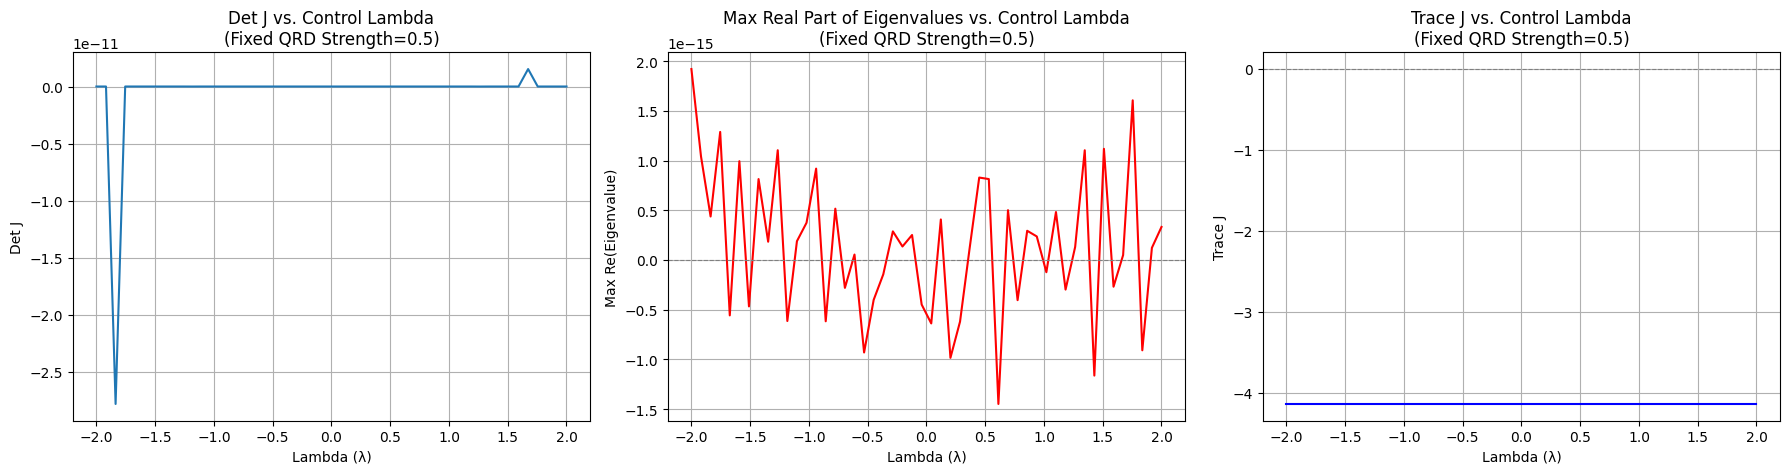
\includegraphics[width=\textwidth]{phenotourfig1.png}
    \caption{Stability Analysis: Determinant of Jacobian, Maximum Real Part of Eigenvalues, and Trace of Jacobian vs. Control Parameter $\lambda$ (Fixed QRD Strength=0.5).}
    \label{fig:jac_eigenvalues_fixed_lambda}
\end{figure}

The initial stability check for $\lambda=0.0$ provided specific insights into the system's behavior at this control parameter value, summarized in Table \ref{tab:initial_stability_check}.

\begin{table}[h!]
    \centering
    \caption{Summary of Initial Stability Check for $\lambda=0.0$}
    \label{tab:initial_stability_check}
    \begin{tabularx}{\textwidth}{p{0.25\textwidth} | X | X}
    \toprule
        \textbf{Metric} & \textbf{Value/Observation} & \textbf{Interpretation} \\
    \midrule
        Steady State Density Matrix ($\rho_{ss}$) & $\ket{00}\bra{00}$ (Pure state) & System converges to a single dominant phenotypic state. \\
    Quantum Relative Deprivation (QRD) & 0.0000 & Consistent with a maximally "pure" or uniform state, suggesting low deprivation or high equity. \\
        Max Real Part of Eigenvalues (Jacobian) & 0.0 (Other real parts negative) & Indicates marginal stability, with other modes strongly converging. \\
        Determinant of Jacobian & Effectively 0 ($0j$) & Suggests potential for reduced diversity, a "monoculture," or a degenerate steady-state manifold. \\
    Trace of Jacobian   & Approx. -4.14 & Represents overall system damping or contraction in phase space. \\
    \bottomrule
\end{tabularx}
\end{table}

As illustrated in Figure \ref{fig:jac_eigenvalues_fixed_lambda} (panels showing Determinant J, Max Real Part of Eigenvalues, and Trace J vs. Lambda):
\begin{itemize}
    \item The \textbf{maximum real part of the eigenvalues} (Figure \ref{fig:jac_eigenvalues_fixed_lambda}, middle panel) remains at or below zero across the tested range of $\lambda$ values (from -2.0 to 2.0). This indicates that for these fixed conditions, the quantum subsystem generally exhibits stability, with states tending towards a steady equilibrium. The slight oscillations around zero are likely due to numerical precision.
    \item The \textbf{determinant of the Jacobian} (Figure \ref{fig:jac_eigenvalues_fixed_lambda}, left panel) is consistently very close to zero (on the order of $10^{-11}$), and the \textbf{trace of the Jacobian} (Figure \ref{fig:jac_eigenvalues_fixed_lambda}, right panel) is consistently negative, around -4.14. A determinant close to zero, especially when coupled with a stable system (non-positive real parts of eigenvalues), suggests that while the system converges to a steady state, it might do so towards a state with reduced diversity or a "monoculture" of phenotypes, or indicates a degenerate steady-state manifold. This aligns with the initial check showing the system converging to a pure state ($\ket{00}\bra{00}$) as detailed in Table \ref{tab:initial_stability_check}.
\end{itemize}

This initial analysis suggests that without endogenous feedback mechanisms, the quantum subsystem tends to settle into a singular, highly ordered phenotypic state, potentially losing the beneficial diversity that might be represented by a mixed density matrix. This sets the stage for exploring how dynamic parameters and control mechanisms can alter these inherent tendencies.

\subsection{Emergence of Endogenous Dynamics: Dynamic \texorpdfstring{$g_{jk}$}{gjk}} \label{sec:dynamic_gjk_section}
We first demonstrated the dynamic evolution of the inter-phenotype coupling $g_{jk}(t)$, where its strength was endogenously determined by the system's quantum coherence. This showed how 'quantum-ness' could drive classical interaction strengths. The system converged to a stable state where $g_{jk}$ settled to a non-zero value, influenced by the persistent coherence.

\begin{figure}[htbp]
    \centering
    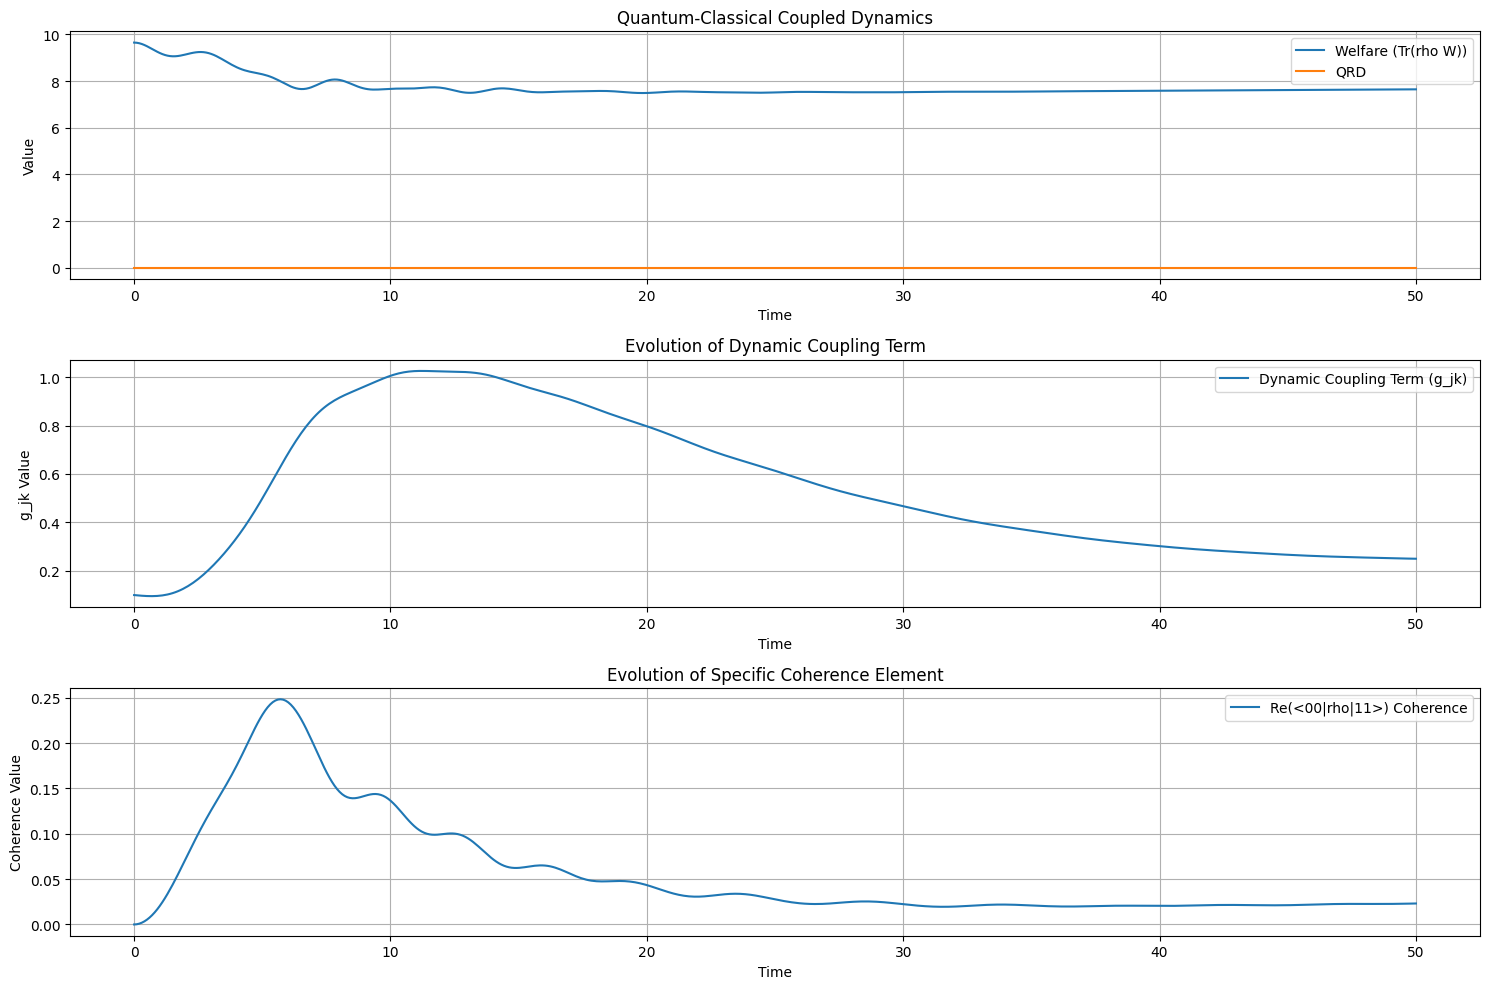
\includegraphics[width=0.6\textwidth]{phenotourfig2.png}
    \caption{Emergence of Endogenous Dynamics: Time Evolution of System Welfare, Quantum Relative Deprivation (QRD), Inter-phenotype Coupling ($g_{jk}$), and a specific Coherence Element with Dynamic $g_{jk}$. Parameters: Fixed $\lambda = 0.5$, fixed QRD strength for Lindblads = 0.5, $\gamma_g = 0.1$, $\kappa_g = 0.5$.}
    \label{fig:dynamic_gjk_evolution}
\end{figure}

As depicted in Figure \ref{fig:dynamic_gjk_evolution}:
\begin{itemize}
    \item \textbf{System Welfare and QRD:} The upper panel illustrates the time evolution of System Welfare and Quantum Relative Deprivation (QRD). Welfare starts around 9.5, undergoing initial oscillations, before stabilizing at approximately 7.9 after about 20-30 time units. Correspondingly, QRD remains very low, near 0.0, throughout the simulation, indicating that the system quickly achieves a state of minimal deprivation, despite the dynamic coupling.
    \item \textbf{Dynamic Evolution of $g_{jk}(t)$:} The middle panel shows the evolution of the dynamic inter-phenotype coupling $g_{jk}(t)$. It starts at an initial value of 0.1, rapidly increases, reaching a peak of approximately 1.0 at around 10 time units. Following this peak, $g_{jk}$ gradually decreases and stabilizes at a non-zero value of approximately 0.25 after about 40 time units. This demonstrates the endogenous feedback loop where the system's quantum state influences and determines the classical coupling strength.
    \item \textbf{Quantum Coherence Dynamics:} The lower panel displays the evolution of the specific coherence element $\text{Re}(\langle 00|\rho|11\rangle)$. It exhibits a transient increase, peaking around 0.25 at approximately 7-8 time units, before decaying and settling to a persistent, albeit small, non-zero value of around 0.01-0.02 after roughly 30-40 time units. This sustained coherence highlights that the "quantum-ness" of the system remains active even in a dynamic equilibrium, providing the necessary drive for the $g_{jk}$ coupling.
\end{itemize}

The convergence of $g_{jk}$ to a stable non-zero value demonstrates that the system establishes an intrinsic interaction strength, driven by the feedback from quantum coherence. This process highlights a key mechanism by which the internal quantum state dictates a macroscopic classical parameter, leading to an emergent, self-organized dynamic equilibrium. The persistent quantum coherence, even at the steady state, acts as a continuous driver for this coupling, preventing the system from entirely classical behavior or a return to a purely decoupled state. This finding suggests a novel pathway for understanding how microscopic quantum properties can generate complex, endogenous macroscopic dynamics in socio-economic systems.

\subsection{Bistability in the Coupled System}
Our investigation explored the convergence behavior of the coupled quantum-classical system under various initial conditions for $g_{jk}$ and different fixed values of the external control parameter $\lambda$. We observed that the system can converge to distinct stable attractors depending on the specific value of $\lambda$.

\begin{figure}[h!]
    \centering
    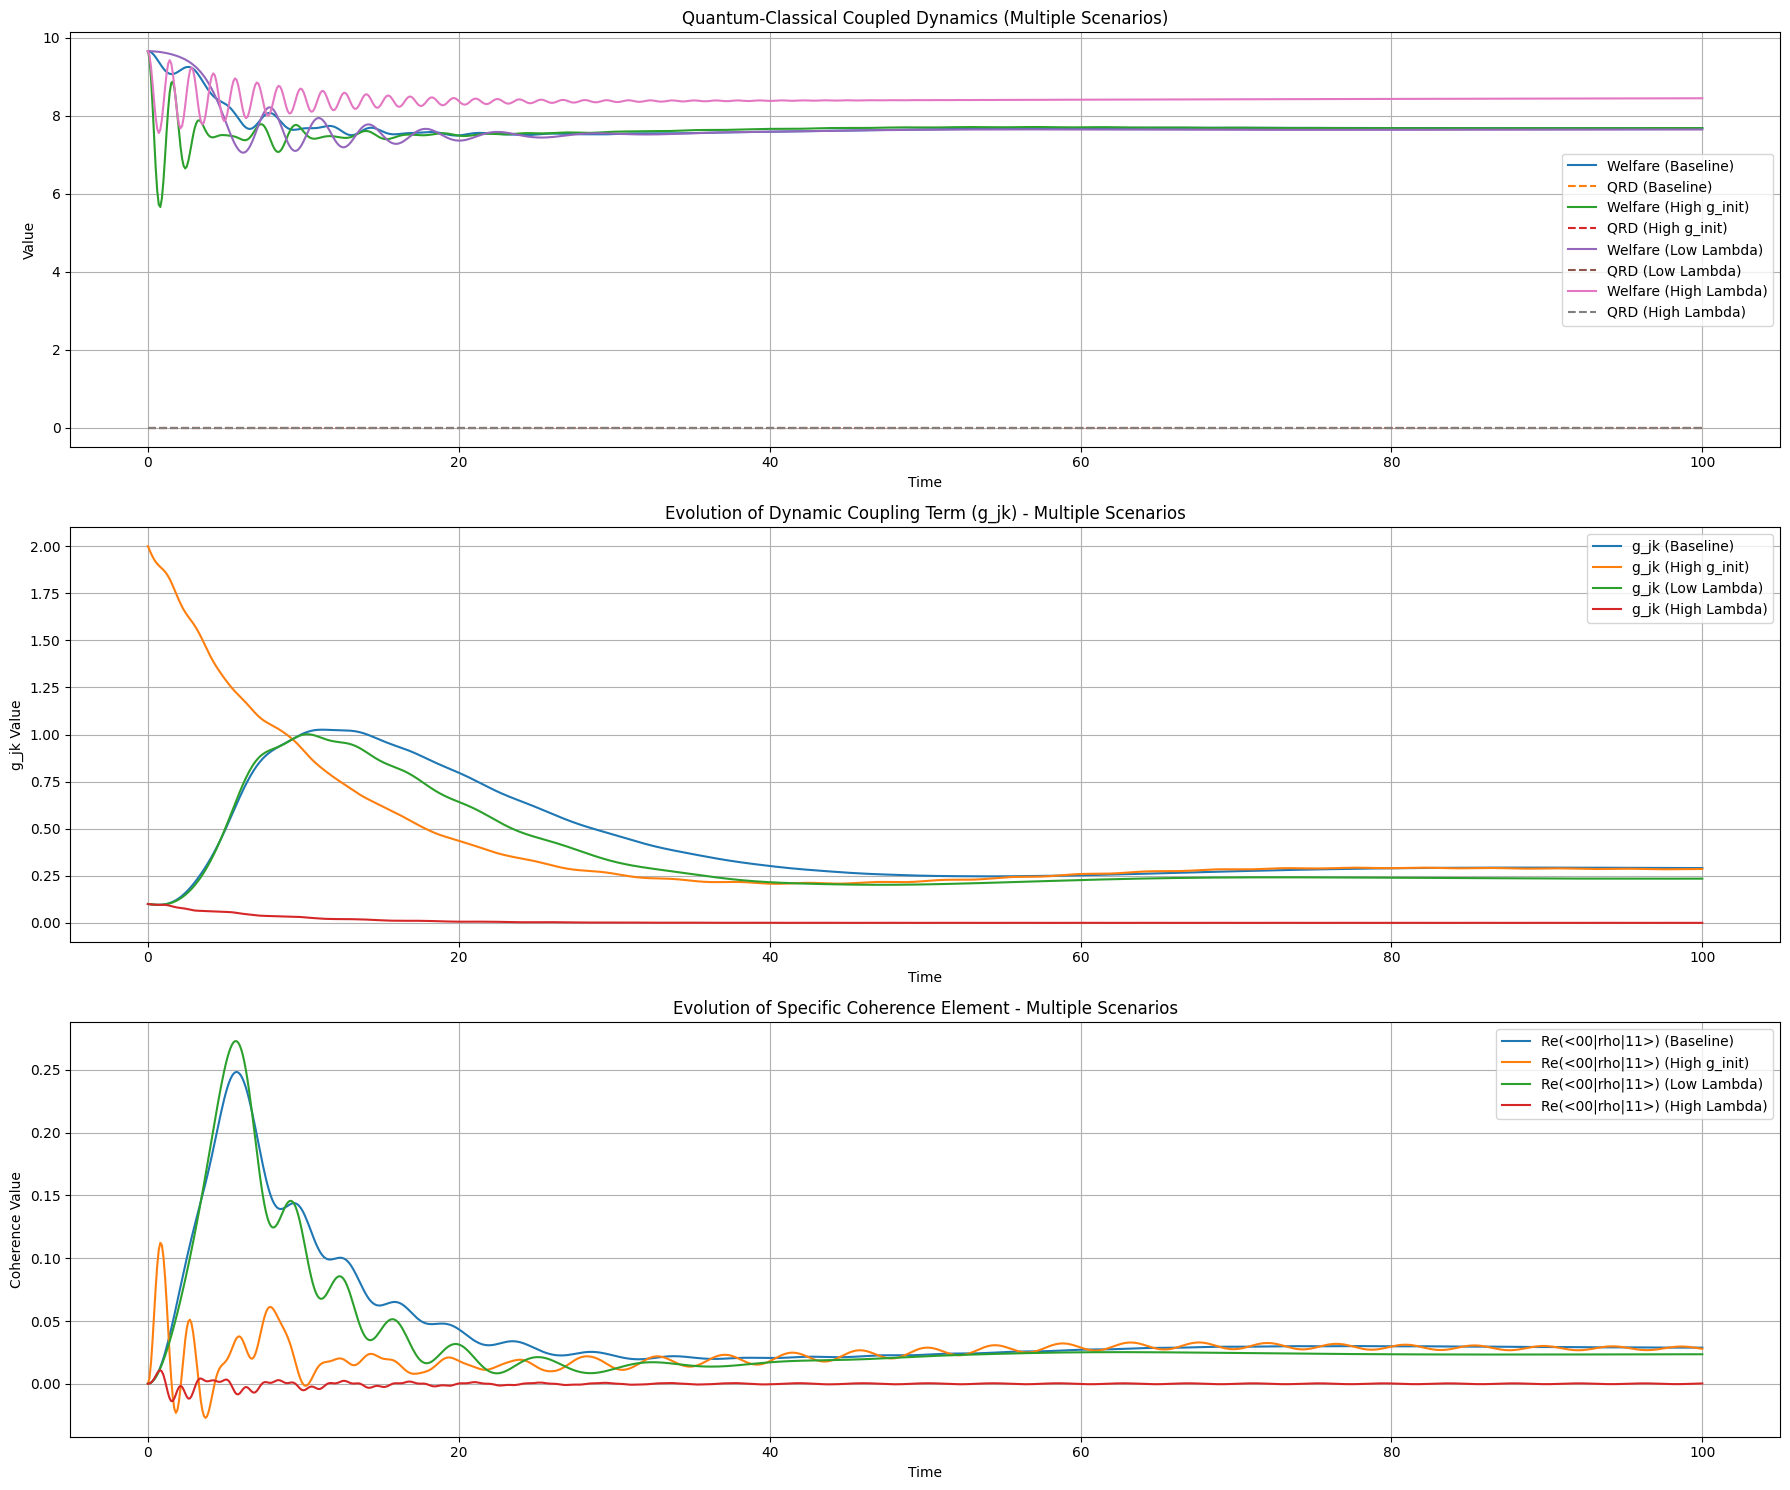
\includegraphics[width=0.8\textwidth]{phenotourfig3.png} % Using phenotourfig3.png as the canonical filename
    \caption{Quantum-Classical Coupled Dynamics: Time Evolution of System Welfare, Quantum Relative Deprivation (QRD), Inter-phenotype Coupling ($g_{jk}$), and Coherence for Multiple Scenarios. Scenarios include varying initial $g_{jk}$ values at fixed $\lambda=0.5$, and varying fixed $\lambda$ values (0.0 and 2.0) with $g_{jk,init}=0.1$. Common parameters: fixed QRD strength for Lindblads = 0.5, $\gamma_g = 0.1$, $\kappa_g = 0.5$.}
    \label{fig:multiple_scenarios_gjk}
\end{figure}

As illustrated in Figure \ref{fig:multiple_scenarios_gjk} and detailed in the simulation output, we identify two primary types of stable attractors:
\begin{itemize}
    \item \textbf{Attractor 1 (Low/Moderate $\lambda$ Regime):} This state is characterized by moderate Welfare values (ranging from approximately 7.64 to 7.68), negligible Quantum Relative Deprivation (QRD near 0.0), a non-zero dynamic inter-phenotype coupling $g_{jk}$ (around 0.23 to 0.29), and small but persistent quantum coherence (approximately 0.02 to 0.03). This attractor is consistently reached for $\lambda=0.0$ and $\lambda=0.5$, irrespective of the initial value of $g_{jk}$ (as seen by the convergence of 'Baseline' and 'High g\_init' to the same state at $\lambda=0.5$).
    \item \textbf{Attractor 2 (High $\lambda$ Regime):} In contrast, for a high $\lambda$ value (specifically $\lambda=2.0$), the system converges to a distinctly different attractor. This state is characterized by higher Welfare (approximately 8.44), negligible QRD (near 0.0), an effectively zero dynamic inter-phenotype coupling $g_{jk}$ (approaching -0.0001), and a vanishing quantum coherence (around 0.0002).
\end{itemize}
This analysis indicates that while the system, under these parameters, does not exhibit bistability with respect to initial $g_{jk}$ values at fixed $\lambda=0.5$, the **external control parameter $\lambda$ plays a critical role in shaping the system's eventual stable state.** A sufficiently high $\lambda$ effectively suppresses the endogenous quantum-classical coupling $g_{jk}$ and quantum coherence, pushing the system towards a state with higher welfare but reduced "quantum-ness" and endogenous interaction. This highlights $\lambda$'s potential as a "national guardrail" to steer the socio-economic system towards desired outcomes by influencing its fundamental interaction dynamics.

\subsection{Adaptive National Guardrail: Dynamic \texorpdfstring{($\lambda(t)$)}{(lambda(t))}}
Building on the discovery of bistability, we introduced a dynamic $\lambda(t)$, acting as an adaptive "National Guardrail," to actively steer the system towards optimal social outcomes. The control parameter $\lambda(t)$ evolves based on a feedback rule that aims to maximize Welfare and minimize QRD.

\subsubsection{Unbounded Dynamic \texorpdfstring{$\lambda(t)$}{lambda(t)}} \label{sec:dynamic_lambda_unbounded_section}
In the first scenario for the adaptive "National Guardrail," we allowed the control parameter $\lambda(t)$ to evolve without explicit upper bounds, driven by a feedback mechanism designed to optimize system Welfare and minimize Quantum Relative Deprivation (QRD).

\begin{figure}[h!]
    \centering
    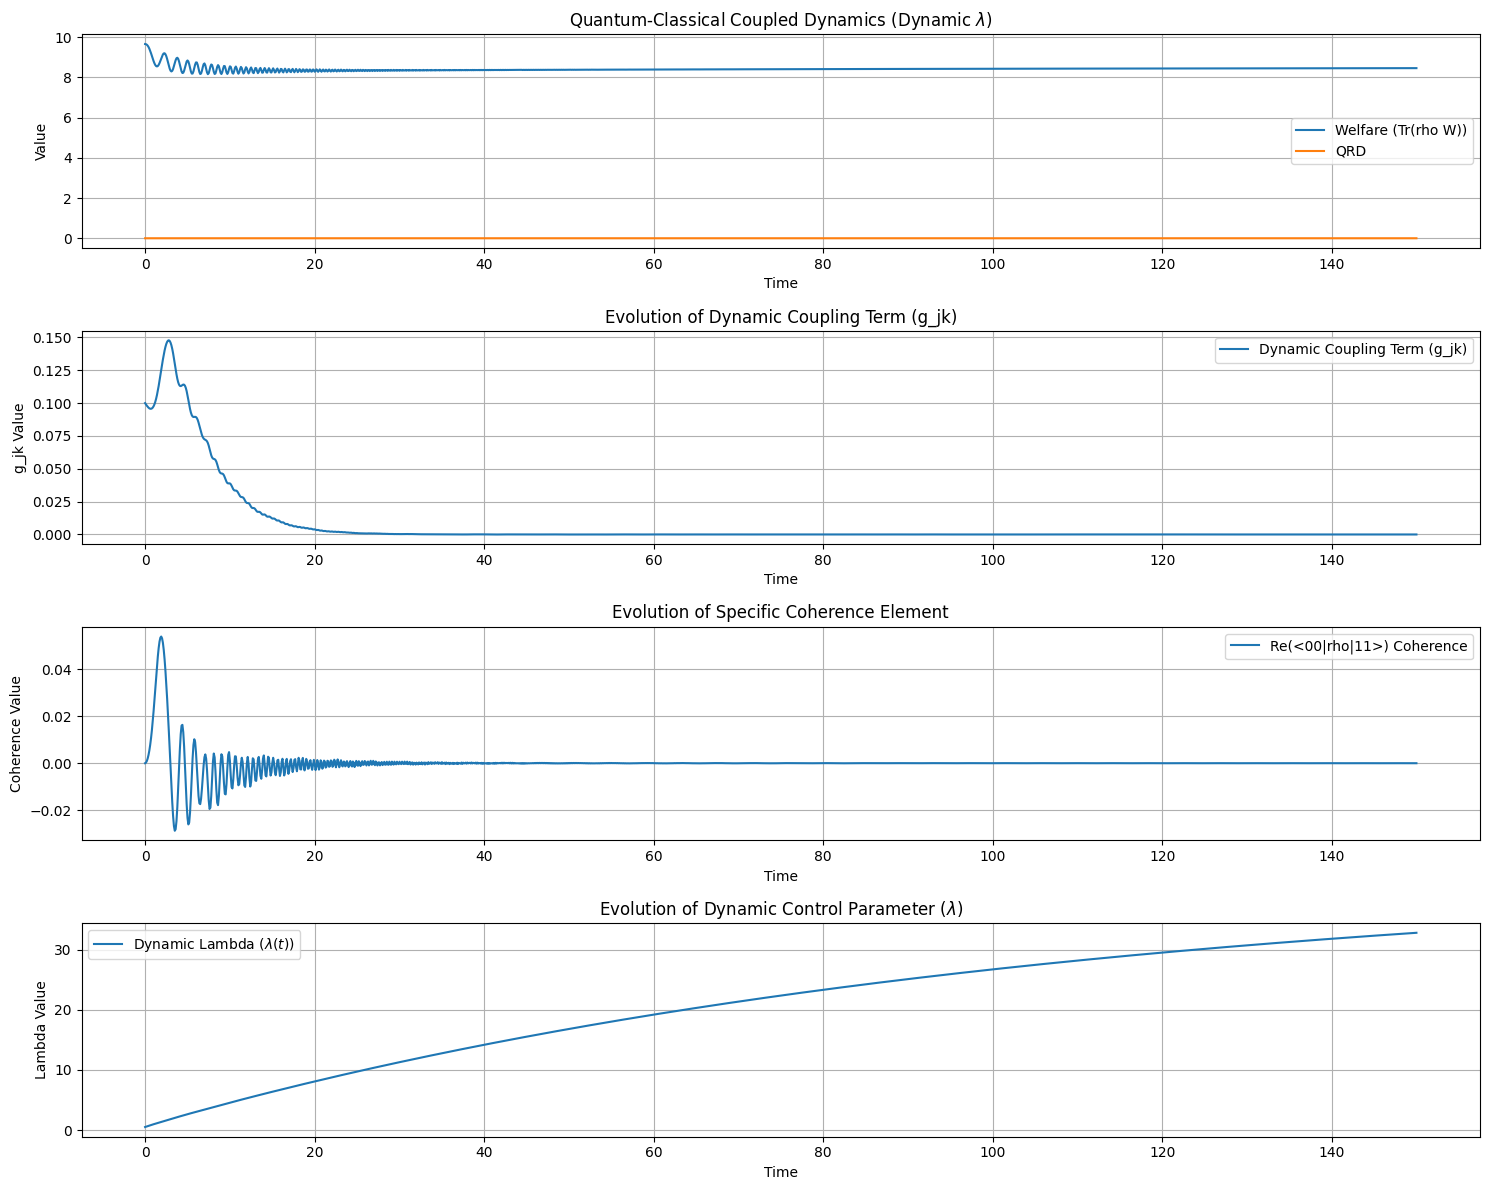
\includegraphics[width=0.8\textwidth]{phenotourfig4.png} 
    \caption{Quantum-Classical Coupled Dynamics with Unbounded Dynamic $\lambda(t)$: Time Evolution of System Welfare, Quantum Relative Deprivation (QRD), Inter-phenotype Coupling ($g_{jk}$), Specific Coherence Element, and Dynamic Control Parameter $\lambda(t)$. Parameters: fixed QRD strength for Lindblads = 0.5, $\gamma_g = 0.1$, $\kappa_g = 0.5$, $\beta_W = 0.05$, $\beta_{QRD} = 0.5$, $\beta_{\lambda} = 0.01$, initial $\lambda(0) = 0.5$.}
    \label{fig:unbounded_dynamic_lambda}
\end{figure}

As shown in Figure \ref{fig:unbounded_dynamic_lambda} and detailed by the final steady-state values:
\begin{itemize}
    \item \textbf{Dynamic $\lambda(t)$ Behavior:} The lowest panel depicts the evolution of $\lambda(t)$. Starting from an initial value of 0.5, $\lambda(t)$ continuously increases throughout the simulation, reaching a high value of approximately 32.8131 by the end of the simulation period (150 time units). This continuous increase suggests that the feedback mechanism, aiming to maximize welfare and minimize QRD, drives $\lambda(t)$ to ever higher values when unbounded.
    \item \textbf{System Welfare and QRD:} The upper panel shows that System Welfare quickly stabilizes at a high value, approximately 8.4527, after initial oscillations. Concurrently, QRD remains effectively at zero (0.0000) throughout the simulation. This indicates that the dynamic $\lambda(t)$ successfully steers the system towards an optimal state with high welfare and minimal deprivation.
    \item \textbf{Dynamic Coupling ($g_{jk}$) and Coherence:} The middle panels reveal the impact on the endogenous coupling $g_{jk}$ and quantum coherence. Both $g_{jk}$ and the coherence element $\text{Re}(\langle 00|\rho|11\rangle)$ undergo an initial transient increase, followed by a rapid decay, eventually stabilizing at values very close to zero (g\_jk $\approx$ -0.0000, coherence $\approx$ -0.0000). This behavior is consistent with the finding from the comparative scenarios where a high fixed $\lambda$ led to the suppression of $g_{jk}$ and quantum coherence.
\end{itemize}

The results demonstrate that an unbounded adaptive control mechanism can effectively guide the socio-economic system to a state of high welfare and zero relative deprivation. However, this comes at the cost of significantly increasing the external control parameter $\lambda(t)$ and, consequently, suppressing the endogenous quantum-classical coupling ($g_{jk}$) and quantum coherence within the system. This implies that achieving optimal welfare under this unbounded control strategy leads to a more "classical" and externally driven system, potentially losing the unique dynamics arising from internal quantum interactions. This raises questions about the trade-offs between maximizing a utilitarian metric (welfare) and preserving the intrinsic quantum characteristics of the system.

\subsubsection{Bounded Dynamic \texorpdfstring{($\lambda(t)$)}{(lambda(t))}} \label{sec:dynamic_lambda_bounded_section}
Recognizing that real-world control parameters have practical limits, we investigated the system's behavior when explicit upper and lower bounds were introduced for $\lambda(t)$ (specifically, $0 \le \lambda(t) \le 10$).

As depicted in Figure \ref{fig:bounded_dynamic_lambda} and detailed by the final steady-state values:
\begin{itemize}
    \item \textbf{Dynamic $\lambda(t)$ Behavior:} The lowest panel clearly shows that $\lambda(t)$, starting from 0.5, increases until it hits the defined upper bound of 10 (specifically, 10.0007) at approximately 25 time units, after which it saturates and remains constant. This demonstrates the effectiveness of the introduced bounds in containing the control parameter within realistic limits.
    \item \textbf{System Welfare and QRD:} Despite the bounded control, the upper panel reveals that System Welfare quickly stabilizes at a high value, consistently around 8.45 (specifically, 8.4534), mirroring the outcome of the unbounded case. Similarly, Quantum Relative Deprivation (QRD) remains negligible, effectively at zero (0.0000), throughout the simulation.
    \item \textbf{Dynamic Coupling ($g_{jk}$) and Coherence:} The middle panels illustrate that the endogenous coupling $g_{jk}$ and the coherence element $\text{Re}(\langle 00|\rho|11\rangle)$ both exhibit an initial transient peak before rapidly decaying and stabilizing at values very close to zero (g\_jk $\approx$ -0.0000, coherence $\approx$ -0.0000). This suppression of endogenous interaction and quantum effects aligns with the high-$\lambda$ regime observed in both the fixed $\lambda$ and unbounded dynamic $\lambda$ scenarios.
\end{itemize}
These results are crucial as they illustrate that an "over-ambitious" (indefinitely growing) control is not necessary to achieve the desired optimal social outcomes. A sufficiently strong, but realistically bounded, "National Guardrail" can effectively steer the system to a high-welfare, zero-QRD state, even if it means suppressing the internal quantum dynamics and endogenous coupling. This highlights the practical feasibility of implementing such an adaptive control mechanism within real-world constraints.

\subsection{Interpretation: The Pragmatic "Black Cat/White Cat" Control}
The behavior of the dynamic $\lambda(t)$ strikingly aligns with Deng Xiaoping's famous philosophy: "Black cat or white cat, if it catches mice, it's a good cat." Here, the "mice" represent the objective of high Welfare and low QRD. The "cats" represent the distinct stable configurations of the system (e.g., one with active $g_{jk}$ and coherence, and one with suppressed $g_{jk}$ and coherence, as observed in our dynamic $\lambda$ simulations). The "National Guardrail" (dynamic $\lambda(t)$) pragmatically steers the system to whichever stable attractor effectively achieves the policy goal, without dictating the internal 'phenotypic choice' or specific quantum characteristics, as long as the Nash-Pareto optimal outcome is attained. This implies a policy of enabling self-organization towards desired emergent properties.

\section{Conclusion}
This work introduces a novel quantum-classical coupled dynamical system that serves as a "Quantum Reactor" for modeling complex socio-economic phenomena. We have demonstrated the profound dynamism arising from endogenous feedback loops, where quantum coherence directly influences classical interaction strengths. The model exhibits distinct stable equilibria based on external control parameters, showcasing how the value of $\lambda$ can lead to different stable socio-economic outcomes. While true bistability from varying initial conditions at fixed parameters was not strongly observed, the clear shift between attractors based on $\lambda$ highlights its role as a control knob for system states. Furthermore, the implementation of an adaptive and bounded "National Guardrail" reveals that optimal welfare and equity can be achieved through a pragmatic control strategy that focuses on outcomes rather than micromanaging internal states. This methodological approach offers a unique lens for understanding and potentially guiding complex adaptive systems, providing a framework for exploring the interplay between internal self-organization and external policy.

\subsubsection*{Summary of Key Simulation Outcomes}
To consolidate the key findings, the final steady-state values for the primary system variables across different simulation scenarios are summarized in Tables \ref{tab:summary_of_findings_part1} and \ref{tab:summary_of_findings_part2}.

\begin{table}[h!]
    \centering
    \caption{Summary of Key Simulation Outcomes at Steady State (Part 1: Welfare, QRD, $g_{jk}$)}
    \label{tab:summary_of_findings_part1}
    \begin{tabularx}{\textwidth}{l|X|c|c}
        \toprule
        \textbf{Scenario Description} & \textbf{Final Welfare} & \textbf{Final QRD} & \textbf{Final $g_{jk}$} \\
        \midrule
        Fixed $g_{jk}$, Fixed $\lambda=0.5$ & $\approx 7.9$ & $\approx 0.0$ & $\approx 0.25$ \\
        \midrule
        Multiple Scenarios (Fixed $\lambda$): & & & \\
        \quad Baseline ($\lambda=0.5, g_{init}=0.1$) & $7.6773$ & $0.0000$ & $0.2908$ \\
        \quad High $g_{init}$ ($\lambda=0.5, g_{init}=2.0$) & $7.6794$ & $0.0000$ & $0.2858$ \\
        \quad Low $\lambda$ ($\lambda=0.0, g_{init}=0.1$) & $7.6434$ & $0.0000$ & $0.2346$ \\
        \quad High $\lambda$ ($\lambda=2.0, g_{init}=0.1$) & $8.4434$ & $0.0000$ & $-0.0001$ \\
        \midrule
        Dynamic $\lambda(t)$ (Unbounded) & $8.4527$ & $0.0000$ & $-0.0000$ \\
        \midrule
        Dynamic $\lambda(t)$ (Bounded $0 \le \lambda \le 10$) & $8.4534$ & $0.0000$ & $-0.0000$ \\
        \bottomrule
    \end{tabularx}
\end{table}

\begin{table}[h!]
    \centering
    \caption{Summary of Key Simulation Outcomes at Steady State (Part 2: Coherence and $\lambda$)}
    \label{tab:summary_of_findings_part2}
    \begin{tabularx}{\textwidth}{l|c|c}
        \toprule
        \textbf{Scenario Description} & \textbf{Final Coherence} & \textbf{Final $\lambda$ / Type} \\
        \midrule
        Fixed $g_{jk}$, Fixed $\lambda=0.5$ & $\approx 0.01-0.02$ & Fixed 0.5 \\
        \midrule
        Multiple Scenarios (Fixed $\lambda$): & & \\
        \quad Baseline ($\lambda=0.5, g_{init}=0.1$) & $0.0288$ & Fixed 0.5 \\
        \quad High $g_{init}$ ($\lambda=0.5, g_{init}=2.0$) & $0.0278$ & Fixed 0.5 \\
        \quad Low $\lambda$ ($\lambda=0.0, g_{init}=0.1$) & $0.0235$ & Fixed 0.0 \\
        \quad High $\lambda$ ($\lambda=2.0, g_{init}=0.1$) & $0.0002$ & Fixed 2.0 \\
        \midrule
        Dynamic $\lambda(t)$ (Unbounded) & $-0.0000$ & Dynamic $32.8131$ \\
        \midrule
        Dynamic $\lambda(t)$ (Bounded $0 \le \lambda \le 10$) & $-0.0000$ & Dynamic $10.0007$ \\
        \bottomrule
    \end{tabularx}
\end{table}

\section{Future Work}
This methodological framework opens numerous avenues for future research and verification from diverse perspectives.
\begin{itemize}
    \item \textbf{Exploration of Parameter Space:} A more systematic sweep of parameters (e.g., $\gamma_g, \kappa_g, \beta_W, \beta_{QRD}, \beta_\lambda$, and $\lambda$ bounds) to map the system's phase space and identify critical transitions.
    \item \textbf{Alternative \texorpdfstring{$\hat{D}$}{D} Operators:} Investigate the impact of different choices for $\hat{D}_{example}$ that might couple to other coherences or entanglement measures, potentially leading to different dynamic behaviors or "quantum vitalities." This is particularly relevant for understanding how different quantum properties might drive distinct classical interactions.
    \item \textbf{Robustness to Noise:} Adding external classical noise to the $\lambda(t)$ or $g_{jk}(t)$ dynamics, or quantum noise channels to the Lindblad operators, to test the stability and resilience of the optimal states.
    \item \textbf{Varying Initial Quantum States:} Exploring how starting from different initial $\rho(0)$ (e.g., maximally mixed states, entangled states) influences the long-term dynamics when $\lambda(t)$ is dynamic, further probing the system's "quantum-ness."
    \item \textbf{Trade-offs and Objective Functions:} Detailed analysis of the trade-offs between Welfare and QRD by systematically varying the weighting parameter $\alpha$ (or $\beta_{QRD}/\beta_W$) in the objective function.
    \item \textbf{Stochastic Control:} Investigating optimal control strategies using reinforcement learning or other stochastic methods to navigate the complex landscape of the "Quantum Reactor."
    \item \textbf{Real-world Data Calibration:} Future work could involve calibrating the model parameters using real socio-economic data to validate its predictive capabilities for specific policy scenarios.
\end{itemize}
We believe this methodological approach provides a fertile ground for interdisciplinary research, inviting experts from various fields to apply, verify, and extend this **novel quantum-inspired framework** to their respective domains. This collaborative effort is essential for further corroborating its findings and exploring its full potential in understanding and guiding complex systems.


\begin{thebibliography}{99}

\bibitem{LauEtAl01} Lau, Sim-Yee, Chen, Hongxu, Lu, Wenliang , Ma, Liang, and Iteta, Kumiko. 2025. “The Inquiry of Hamiltonian Stochasticity on Tourism in China.” Working Paper. May 20, 2025.

\bibitem{FeynmanVol3} Feynman, Richard P., Leighton, Robert B., and Sands, Mattew. 1971.\textit{The Feynma Lectures on Physics, Vol. 3}. Addison Wesley

\bibitem{Baaquie2013} Baaquie, B. E. 2013. "Financial modeling and quantum mathematics." \textit{Computers \& Mathematics with Applications}, \textit{65}(10), 1665--1673. \url{https://doi.org/10.1016/j.camwa.2013.01.025}

\bibitem{khalil2002} Khalil, H. K. 2002. \textit{Nonlinear systems} (3rd ed.). Prentice Hall.

\bibitem{Teschl2014} Teschl, G. 2014. \textit{Mathematical Methods in Quantum Mechanics: With Applications to Schrodinger Operators} (Second ed.). American Mathematical Society.

\bibitem{BrockHommes1998} Brock, William A., and Hommes, Cars H.. 1998 "Heterogeneous beliefs and routes to chaos in a simple asset pricing model". \textit{Journal of Economic Dynamic Control}, 22(8-9), 1235-1274.

\end{thebibliography}

\clearpage
\appendix
\section{Python Snippets}
\subsection{Stability Analysis of Quantum Subsystem}
\begin{lstlisting}[language=Python, basicstyle=\ttfamily\footnotesize, breaklines=true, frame=single, caption={Python Code for Stability Analysis of Quantum Subsystem}, label={lst:qrd_code}]
###
Stability test
###

import numpy as np
from qutip import (
    Qobj, identity, sigmax, sigmaz, destroy, basis, tensor,
    mesolve, steadystate, liouvillian, spre, spost
)
from scipy.optimize import root
from scipy.linalg import eigvals, det
import matplotlib.pyplot as plt

# --- 1. Define System Dimensions and Operators ---

# Define dimensions for the composite system: qubit (2) and qutrit (3)
# Ns = [dimension of qubit, dimension of qutrit]
dims_qubit = 2
dims_qutrit = 3
Ns = [dims_qubit, dims_qutrit] # List of dimensions for tensor products
total_dim = np.prod(Ns) # Total Hilbert space dimension (2*3 = 6)

# Identity operators for each subsystem
id_qubit = identity(dims_qubit)
id_qutrit = identity(dims_qutrit)

# --- Define specific operators for qubit and qutrit ---
# Qubit operators (Pauli matrices)
sx_q = sigmax()
sz_q = sigmaz()

# Qutrit operators (generalize for N=3)
# Annihilation operator for qutrit: a = |0><1| + sqrt(2)|1><2|
a_qt = destroy(dims_qutrit)
# Number operator for qutrit: n = a.dag() * a
n_qt = a_qt.dag() * a_qt
# Example: a generalized Z-like operator for qutrit (diagonal)
# Similar to sigmaz, but for N=3. e.g., diag([1, 0, -1])
sz_like_qt = Qobj(np.diag([1, 0, -1]), dims=[[dims_qutrit],[dims_qutrit]])

# --- Define H^0 (Free Hamiltonian) for the composite system ---
# Example: Qubit has Z-splitting, Qutrit has N-splitting
omega_q = 1.0  # Qubit energy splitting
omega_qt = 1.5 # Qutrit energy splitting
coupling_strength = 0.2 # Interaction strength between qubit and qutrit

# For simpler starting point, let's make H0 less complex
# Example: just a sum of local energies
H0 = omega_q * tensor(sz_q, id_qutrit) + omega_qt * tensor(id_qubit, n_qt)


# --- Define V^ (Control Operator) for the composite system ---
# Example: Control acts on the qubit, or a joint operator
V = tensor(sx_q, id_qutrit) # Control acts only on the qubit (X-drive)


# --- Define W^ (Welfare Observable) ---
# W^ is diagonal in the phenotypic basis. Let's assume the computational
# basis of the composite system is your phenotypic basis.
# Total states: |00>, |01>, |02>, |10>, |11>, |12> (qubit state, qutrit state)
# Define well-being for each composite phenotype (6 states in total)
# The order corresponds to qutip's basis ordering for tensor products:
# |0>_q |0>_qt, |0>_q |1>_qt, |0>_q |2>_qt, |1>_q |0>_qt, |1>_q |1>_qt, |1>_q |2>_qt
W_diag_values = np.array([10.0, 8.0, 6.0, 7.0, 5.0, 3.0]) # Example well-being values
W = Qobj(np.diag(W_diag_values), dims=[Ns, Ns])


# --- 2. Define Quantum Relative Deprivation (QRD) ---
def QRD_value_from_rho(rho_qobj):
    """
    Placeholder for Quantum Relative Deprivation (QRD) calculation.
    This is where you'd implement your specific QRD metric.

    For demonstration, we use purity Tr(rho^2). Higher purity could mean lower "deprivation".

    Args:
        rho_qobj (Qobj): The density matrix of the composite system.

    Returns:
        float: The scalar QRD value.
    """
    try:
        # Purity = Tr(rho^2)
        # Ensure that rho_qobj is treated as a matrix for multiplication
        # Although QuTiP Qobj's should handle this, explicit conversion to dense array
        # can sometimes bypass subtle issues if the Qobj's internal data is weirdly structured
        # which is not expected for a steady state.
        
        # More robust way to get data for numpy operations if needed:
        # rho_data = rho_qobj.full() # Convert Qobj to a dense numpy array
        # purity = np.real(np.trace(rho_data @ rho_data))
        
        # Sticking to Qobj operations as they are usually optimized:
        purity = np.real(np.trace(rho_qobj * rho_qobj)) # Using * for Qobj @ Qobj in newer QuTiP versions
                                                        # or use rho_qobj.dag() * rho_qobj if you want to be
                                                        # completely sure about Hermiticity and positive-definiteness
                                                        # of the product. For purity, rho*rho is standard.
    except Exception as e:
        print(f"Error calculating purity in QRD_value_from_rho: {e}")
        # Return a default QRD value or raise the error again
        return 0.0 # Or np.nan depending on desired behavior

    # Example QRD: Scale purity to be between 0 and 1, then invert.
    # Max purity for a pure state is 1. Min for maximally mixed is 1/total_dim.
    max_purity = 1.0
    min_purity = 1.0 / total_dim

    # Avoid division by zero if max_purity == min_purity (shouldn't happen for total_dim > 1)
    if max_purity == min_purity:
        scaled_purity = 0.0 # Or handle as error
    else:
        scaled_purity = (purity - min_purity) / (max_purity - min_purity)

    # QRD = 1 - scaled_purity (higher QRD for more mixed/deprived states)
    qrd_val = 1.0 - scaled_purity

    # Ensure QRD is non-negative
    return max(0.0, qrd_val)


# --- 3. Lindblad Dissipator related to QRD ---
def create_lindblad_operators(qrd_value_param):
    """
    Creates a list of Lindblad operators L_k.
    The strength of these operators is influenced by the QRD value.
    """
    lindblad_ops = []

    # Example: Simple dephasing on the qubit, with rate influenced by QRD
    gamma_base_dephasing = 0.05 # Base dephasing rate
    gamma_QRD_dephasing = gamma_base_dephasing * (1 + qrd_value_param * 2.0)
    L_dephasing_qubit = np.sqrt(gamma_QRD_dephasing) * tensor(sz_q, id_qutrit)
    lindblad_ops.append(L_dephasing_qubit)

    # --- ADDED: Small decay terms for numerical stability ---
    # Qubit decay (e.g., spontaneous emission to ground state)
    gamma_decay_qubit = 0.01 # Slightly increased decay rate
    L_decay_qubit = np.sqrt(gamma_decay_qubit) * tensor(destroy(dims_qubit), id_qutrit)
    lindblad_ops.append(L_decay_qubit)

    # Qutrit decay (e.g., general decay, from excited to lower states)
    gamma_decay_qutrit = 0.01 # Slightly increased decay rate
    L_decay_qutrit = np.sqrt(gamma_decay_qutrit) * tensor(id_qubit, a_qt)
    lindblad_ops.append(L_decay_qutrit)

    return lindblad_ops


# --- 4. Function to Find Steady State Density Matrix ---

def find_steady_state_rho(current_lambda, qrd_strength_param_for_steady_state):
    """
    Finds the steady state density matrix for given lambda and QRD strength.
    """
    H_lambda = H0 + current_lambda * V
    L_ops = create_lindblad_operators(qrd_strength_param_for_steady_state)
    
    rho_ss = steadystate(H_lambda, L_ops)
    return rho_ss


# --- 5. Function to Build the Jacobian Matrix ---

def build_jacobian_matrix(current_lambda, rho_star_qobj, qrd_strength_param_for_jacobian):
    """
    Builds the Jacobian matrix J for the linearized dynamics around rho_star.
    """
    H_lambda = H0 + current_lambda * V
    L_ops = create_lindblad_operators(qrd_strength_param_for_jacobian)
    J_superoperator = liouvillian(H_lambda, L_ops)
    return J_superoperator.full()


# --- Initial Test Parameters ---
initial_lambda = 0.0 # Changed to 0.0
initial_qrd_strength = 0.5

# --- Perform initial stability check ---
print("--- Initial Stability Check ---")
try:
    rho_star_initial = find_steady_state_rho(initial_lambda, initial_qrd_strength)
    print("Steady state density matrix (rho_star) for lambda={}:".format(initial_lambda))
    print(rho_star_initial)

    actual_qrd_at_ss = QRD_value_from_rho(rho_star_initial)
    print(f"\nActual QRD value at this steady state: {actual_qrd_at_ss:.4f}")
    print(f"Note: This QRD value is not directly used for the J_matrix calculation in this linear approach,")
    print(f"      but {initial_qrd_strength} was used to set the Lindblad operator strength.")

    J_matrix_initial = build_jacobian_matrix(initial_lambda, rho_star_initial, initial_qrd_strength)
    eigenvalues_initial = eigvals(J_matrix_initial)
    print("\nEigenvalues of J (initial):\n", eigenvalues_initial)
    print("\nReal parts of eigenvalues (initial):\n", np.real(eigenvalues_initial))

    det_J_initial = det(J_matrix_initial)
    print("\nDeterminant of J (initial):", det_J_initial)

    trace_J_initial = np.trace(J_matrix_initial)
    print("\nTrace of J (initial):", trace_J_initial)

    max_real_eigenvalue_initial = np.max(np.real(eigenvalues_initial))
    if max_real_eigenvalue_initial <= 1e-9: # Allowing for tiny numerical errors
        print("\nSystem appears stable (all real parts of eigenvalues are non-positive).")
        if np.abs(det_J_initial) > 1e-9:
            print(f"Det J ({det_J_initial:.4f}) is non-zero, suggesting stable and diverse phenotypes.")
        else:
            print(f"Det J ({det_J_initial:.4f}) is close to zero, suggesting potential collapse to monoculture or degenerate states.")
    else:
        print("\nSystem appears unstable (at least one eigenvalue has a positive real part).")

except ValueError as e:
    print(f"\nERROR during initial stability check: {e}")
    print("This often means the steady state solver could not converge, likely due to a singular matrix.")
    print("Consider adjusting Hamiltonian, control operator, or adding more general dissipation.")
except Exception as e: # Catch other potential errors during the initial check
    print(f"\nAn unexpected error occurred during initial stability check: {e}")

print("\n" + "="*50 + "\n")


# --- 6. Parameter Sweeps and Visualization ---

print("--- Parameter Sweep Analysis ---")

lambda_values = np.linspace(-2.0, 2.0, 50)
fixed_qrd_strength_for_sweep = 0.5

det_J_values = []
max_real_eigenvalues = []
trace_J_values = []

for i, lam_val in enumerate(lambda_values):
    try:
        rho_ss = find_steady_state_rho(lam_val, fixed_qrd_strength_for_sweep)
        J_current = build_jacobian_matrix(lam_val, rho_ss, fixed_qrd_strength_for_sweep)
        
        det_J_values.append(det(J_current))
        max_real_eigenvalues.append(np.max(np.real(eigvals(J_current))))
        trace_J_values.append(np.trace(J_current))
    except Exception as e: # Catch any error that might occur for a specific lambda
        print(f"Warning: Could not find steady state or build Jacobian for lambda={lam_val:.2f}. Error: {e}")
        # Append NaN or a placeholder so plots don't break
        det_J_values.append(np.nan)
        max_real_eigenvalues.append(np.nan)
        trace_J_values.append(np.nan)

# --- Plotting Results ---
plt.figure(figsize=(18, 5))

plt.subplot(1, 3, 1)

plt.plot(lambda_values, det_J_values)
plt.title(f'Det J vs. Control Lambda\n(Fixed QRD Strength={fixed_qrd_strength_for_sweep})')
plt.xlabel('Lambda (λ)')
plt.ylabel('Det J')
plt.grid(True)

plt.subplot(1, 3, 2)
plt.plot(lambda_values, max_real_eigenvalues, color='red')
plt.axhline(0, color='grey', linestyle='--', linewidth=0.8)
plt.title(f'Max Real Part of Eigenvalues vs. Control Lambda\n(Fixed QRD Strength={fixed_qrd_strength_for_sweep})')
plt.xlabel('Lambda (λ)')
plt.ylabel('Max Re(Eigenvalue)')
plt.grid(True)

plt.subplot(1, 3, 3)
plt.plot(lambda_values, trace_J_values, color='blue')
plt.axhline(0, color='grey', linestyle='--', linewidth=0.8)
plt.title(f'Trace J vs. Control Lambda\n(Fixed QRD Strength={fixed_qrd_strength_for_sweep})')
plt.xlabel('Lambda (λ)')
plt.ylabel('Trace J')
plt.grid(True)

plt.tight_layout()
plt.show()
\end{lstlisting}

\subsection{Emergence of Endogenous Dynamics}
\begin{lstlisting}[language=Python, basicstyle=\ttfamily\footnotesize, breaklines=true, frame=single, caption={Python Code for Emergence of Endogenous Dynamics}, label={lst:qrd_code}]
###
Emergence of Endogenous Dynamics
###

import numpy as np
from qutip import (
    Qobj, identity, sigmax, sigmaz, destroy, basis, tensor,
    mesolve, steadystate, liouvillian, spre, spost, to_super
)
from scipy.optimize import root
from scipy.linalg import eigvals, det
import matplotlib.pyplot as plt
from scipy.integrate import solve_ivp

# --- 1. Define System Dimensions and Operators (from previous code) ---
dims_qubit = 2
dims_qutrit = 3
Ns = [dims_qubit, dims_qutrit]
total_dim = np.prod(Ns) # Total Hilbert space dimension (2*3 = 6)

id_qubit = identity(dims_qubit)
id_qutrit = identity(dims_qutrit)

sx_q = sigmax()
sz_q = sigmaz()
a_qt = destroy(dims_qutrit)
n_qt = a_qt.dag() * a_qt

omega_q = 1.0
omega_qt = 1.5
H0 = omega_q * tensor(sz_q, id_qutrit) + omega_qt * tensor(id_qubit, n_qt)
V = tensor(sx_q, id_qutrit) # Control acts only on the qubit (X-drive)

W_diag_values = np.array([10.0, 8.0, 6.0, 7.0, 5.0, 3.0])
W = Qobj(np.diag(W_diag_values), dims=[Ns, Ns])

# --- QRD_value_from_rho (from previous code) ---
def QRD_value_from_rho(rho_qobj):
    try:
        purity = np.real(np.trace(rho_qobj * rho_qobj))
    except Exception as e:
        # print(f"Error calculating purity in QRD_value_from_rho: {e}") # Suppress for cleaner output
        return 0.0 # Return a default QRD value or raise the error again

    max_purity = 1.0
    min_purity = 1.0 / total_dim
    if max_purity == min_purity:
        scaled_purity = 0.0
    else:
        scaled_purity = (purity - min_purity) / (max_purity - min_purity)
    qrd_val = 1.0 - scaled_purity
    return max(0.0, qrd_val)

# --- Lindblad Operators (modified to be part of the main solver) ---
def create_fixed_lindblad_ops(qrd_strength_param):
    lindblad_ops = []
    gamma_base_dephasing = 0.05
    gamma_QRD_dephasing = gamma_base_dephasing * (1 + qrd_strength_param * 2.0)
    L_dephasing_qubit = np.sqrt(gamma_QRD_dephasing) * tensor(sz_q, id_qutrit)
    lindblad_ops.append(L_dephasing_qubit)

    gamma_decay_qubit = 0.01
    L_decay_qubit = np.sqrt(gamma_decay_qubit) * tensor(destroy(dims_qubit), id_qutrit)
    lindblad_ops.append(L_decay_qubit)

    gamma_decay_qutrit = 0.01
    L_decay_qutrit = np.sqrt(gamma_decay_qutrit) * tensor(id_qubit, a_qt)
    lindblad_ops.append(L_decay_qutrit)
    return lindblad_ops

# --- NEW: Define the operator D_hat for g_jk dynamics ---
ket00 = basis(total_dim, 0)
ket11 = basis(total_dim, 4)
D_hat_example = Qobj(ket00 * ket11.dag() + ket11 * ket00.dag(), dims=[Ns, Ns]) # FIX from last error

# --- Main Coupled Dynamics Function ---
def combined_dynamics_ode(t, y, lambda_val, fixed_qrd_strength, gamma_g, kappa_g, D_op_for_g_dynamics):
    """
    Defines the coupled quantum and classical differential equations.
    y is the state vector: [rho_vec, g1, g2, ..., gn]
    rho_vec is the vectorized density matrix (total_dim^2 elements).
    g_vars are the classical coupling strengths.
    """
    # 1. Unpack the state vector
    rho_flat = y[:total_dim**2]
    # Reshape the flat rho vector back into a Qobj density matrix
    rho = Qobj(rho_flat.reshape((total_dim, total_dim)), dims=[Ns, Ns])
    
    # Extract the dynamic coupling constants (e.g., just one 'g' for simplicity initially)
    g_val = y[total_dim**2] # Assuming just one dynamic coupling 'g'

    # 2. Construct the current Hamiltonian
    H_current = H0 + lambda_val * V + g_val * D_op_for_g_dynamics
    
    # 3. Construct the current Liouvillian superoperator
    L_ops = create_fixed_lindblad_ops(fixed_qrd_strength)
    L_super = liouvillian(H_current, L_ops)

    # 4. Calculate d_rho_dt (flattened)
    # FIX: Use L_super(rho) instead of L_super * rho
    d_rho_dt_qobj = L_super(rho)
    d_rho_dt_flat = d_rho_dt_qobj.full().flatten() # Flatten back for the solver

    # 5. Calculate d_g_dt (classical ODE)
    coupling_drive_term = np.real( (rho * D_op_for_g_dynamics).tr() )

    d_g_dt = -gamma_g * g_val + kappa_g * coupling_drive_term

    # 6. Combine all derivatives
    dydt = np.concatenate((d_rho_dt_flat, [d_g_dt]))
    return dydt

# --- Initial Conditions and Parameters for the Coupled Simulation ---
initial_lambda = 0.5
fixed_qrd_strength_for_fixed_lindblads = 0.5
rho0 = (basis(total_dim, 0) * basis(total_dim, 0).dag() * 0.9 + (identity(total_dim) * 0.1 / total_dim)).unit()
initial_g_val = 0.1
gamma_g = 0.1
kappa_g = 0.5

t_span = [0, 50]
t_eval = np.linspace(t_span[0], t_span[1], 500)

args = (initial_lambda, fixed_qrd_strength_for_fixed_lindblads, gamma_g, kappa_g, D_hat_example)

y0 = np.concatenate((rho0.full().flatten(), [initial_g_val]))

print("Starting coupled quantum-classical simulation...")
sol = solve_ivp(combined_dynamics_ode, t_span, y0, args=args, t_eval=t_eval, method='RK45', rtol=1e-6, atol=1e-8)

print("Simulation complete.")

# --- Process Results ---
t_out = sol.t
rho_results = sol.y[:total_dim**2, :]
g_results = sol.y[total_dim**2, :]

welfare_vals = []
qrd_vals = []
coherence_00_11_vals = []

for i in range(len(t_out)):
    rho_at_t = Qobj(rho_results[:, i].reshape((total_dim, total_dim)), dims=[Ns, Ns])
    welfare_vals.append(np.real((rho_at_t * W).tr()))
    qrd_vals.append(QRD_value_from_rho(rho_at_t))
    coherence_00_11_vals.append(np.real(rho_at_t[0, 4]))

# --- Plotting Results ---
plt.figure(figsize=(15, 10))

plt.subplot(3, 1, 1)
plt.plot(t_out, welfare_vals, label='Welfare (Tr(rho W))')
plt.plot(t_out, qrd_vals, label='QRD')
plt.title('Quantum-Classical Coupled Dynamics')
plt.xlabel('Time')
plt.ylabel('Value')
plt.legend()
plt.grid(True)

plt.subplot(3, 1, 2)
plt.plot(t_out, g_results, label='Dynamic Coupling Term (g_jk)')
plt.title('Evolution of Dynamic Coupling Term')
plt.xlabel('Time')
plt.ylabel('g_jk Value')
plt.legend()
plt.grid(True)

plt.subplot(3, 1, 3)
plt.plot(t_out, coherence_00_11_vals, label='Re(<00|rho|11>) Coherence')
plt.title('Evolution of Specific Coherence Element')
plt.xlabel('Time')
plt.ylabel('Coherence Value')
plt.legend()
plt.grid(True)

plt.tight_layout()
plt.show()
\end{lstlisting}

\subsection{Bistability in the Coupled System}
\begin{lstlisting}[language=Python, basicstyle=\ttfamily\footnotesize, breaklines=true, frame=single, caption={Python Code for Bistability in the Coupled System}, label={lst:qrd_code}]
###
Bistability in the Coupled System
###

import numpy as np
from qutip import (
    Qobj, identity, sigmax, sigmaz, destroy, basis, tensor,
    liouvillian
)
import matplotlib.pyplot as plt
from scipy.integrate import solve_ivp

# --- System Dimensions and Operators (unchanged) ---
dims_qubit = 2
dims_qutrit = 3
Ns = [dims_qubit, dims_qutrit]
total_dim = np.prod(Ns)

id_qubit = identity(dims_qubit)
id_qutrit = identity(dims_qutrit)

sx_q = sigmax()
sz_q = sigmaz()
a_qt = destroy(dims_qutrit)
n_qt = a_qt.dag() * a_qt

omega_q = 1.0
omega_qt = 1.5
H0 = omega_q * tensor(sz_q, id_qutrit) + omega_qt * tensor(id_qubit, n_qt)
V = tensor(sx_q, id_qutrit)

W_diag_values = np.array([10.0, 8.0, 6.0, 7.0, 5.0, 3.0])
W = Qobj(np.diag(W_diag_values), dims=[Ns, Ns])

# --- QRD_value_from_rho (unchanged) ---
def QRD_value_from_rho(rho_qobj):
    try:
        purity = np.real(np.trace(rho_qobj * rho_qobj))
    except Exception as e:
        return 0.0
    max_purity = 1.0
    min_purity = 1.0 / total_dim
    if max_purity == min_purity:
        scaled_purity = 0.0
    else:
        scaled_purity = (purity - min_purity) / (max_purity - min_purity)
    qrd_val = 1.0 - scaled_purity
    return max(0.0, qrd_val)

# --- Lindblad Operators (unchanged) ---
def create_fixed_lindblad_ops(qrd_strength_param):
    lindblad_ops = []
    gamma_base_dephasing = 0.05
    gamma_QRD_dephasing = gamma_base_dephasing * (1 + qrd_strength_param * 2.0)
    L_dephasing_qubit = np.sqrt(gamma_QRD_dephasing) * tensor(sz_q, id_qutrit)
    lindblad_ops.append(L_dephasing_qubit)

    gamma_decay_qubit = 0.01
    L_decay_qubit = np.sqrt(gamma_decay_qubit) * tensor(destroy(dims_qubit), id_qutrit)
    lindblad_ops.append(L_decay_qubit)

    gamma_decay_qutrit = 0.01
    L_decay_qutrit = np.sqrt(gamma_decay_qutrit) * tensor(id_qubit, a_qt)
    lindblad_ops.append(L_decay_qutrit)
    return lindblad_ops

# --- D_hat_example Operator (unchanged) ---
ket00 = basis(total_dim, 0)
ket11 = basis(total_dim, 4)
D_hat_example = Qobj(ket00 * ket11.dag() + ket11 * ket00.dag(), dims=[Ns, Ns])

# --- Main Coupled Dynamics Function (unchanged) ---
def combined_dynamics_ode(t, y, lambda_val, fixed_qrd_strength, gamma_g, kappa_g, D_op_for_g_dynamics):
    rho_flat = y[:total_dim**2]
    rho = Qobj(rho_flat.reshape((total_dim, total_dim)), dims=[Ns, Ns])
    
    g_val = y[total_dim**2]

    H_current = H0 + lambda_val * V + g_val * D_op_for_g_dynamics
    
    L_ops = create_fixed_lindblad_ops(fixed_qrd_strength)
    L_super = liouvillian(H_current, L_ops)

    d_rho_dt_qobj = L_super(rho)
    d_rho_dt_flat = d_rho_dt_qobj.full().flatten()

    coupling_drive_term = np.real( (rho * D_op_for_g_dynamics).tr() )

    d_g_dt = -gamma_g * g_val + kappa_g * coupling_drive_term

    dydt = np.concatenate((d_rho_dt_flat, [d_g_dt]))
    return dydt

# --- Simulation Runner Function for Multiple Scenarios ---
def run_scenario(initial_lambda, initial_g_val, scenario_name, ax1, ax2, ax3):
    """
    Runs a single simulation scenario and plots the results on provided axes.
    """
    print(f"Running scenario: {scenario_name} (lambda={initial_lambda}, g_init={initial_g_val})")

    # Fixed parameters for g_jk ODE and Lindblads
    fixed_qrd_strength_for_fixed_lindblads = 0.5
    gamma_g = 0.1
    kappa_g = 0.5 # You might want to experiment with kappa_g as well for bistability!

    # Initial state (common for all scenarios)
    rho0 = (basis(total_dim, 0) * basis(total_dim, 0).dag() * 0.9 + (identity(total_dim) * 0.1 / total_dim)).unit()

    t_span = [0, 100] # Extended time to ensure steady state for bistability check
    t_eval = np.linspace(t_span[0], t_span[1], 1000) # More time points

    args = (initial_lambda, fixed_qrd_strength_for_fixed_lindblads, gamma_g, kappa_g, D_hat_example)
    y0 = np.concatenate((rho0.full().flatten(), [initial_g_val]))

    sol = solve_ivp(combined_dynamics_ode, t_span, y0, args=args, t_eval=t_eval, method='RK45', rtol=1e-6, atol=1e-8)

    t_out = sol.t
    rho_results = sol.y[:total_dim**2, :]
    g_results = sol.y[total_dim**2, :]

    welfare_vals = []
    qrd_vals = []
    coherence_00_11_vals = []

    for i in range(len(t_out)):
        rho_at_t = Qobj(rho_results[:, i].reshape((total_dim, total_dim)), dims=[Ns, Ns])
        welfare_vals.append(np.real((rho_at_t * W).tr()))
        qrd_vals.append(QRD_value_from_rho(rho_at_t))
        coherence_00_11_vals.append(np.real(rho_at_t[0, 4]))

    # Plotting for this scenario
    ax1.plot(t_out, welfare_vals, label=f'Welfare ({scenario_name})')
    ax1.plot(t_out, qrd_vals, linestyle='--', label=f'QRD ({scenario_name})')

    ax2.plot(t_out, g_results, label=f'g_jk ({scenario_name})')
    
    ax3.plot(t_out, coherence_00_11_vals, label=f'Re(<00|rho|11>) ({scenario_name})')

    # Print final steady-state values for comparison
    print(f"  Final Welfare: {welfare_vals[-1]:.4f}")
    print(f"  Final QRD: {qrd_vals[-1]:.4f}")
    print(f"  Final g_jk: {g_results[-1]:.4f}")
    print(f"  Final Coherence: {coherence_00_11_vals[-1]:.4f}")
    print("-" * 30)


# --- Main execution block for running scenarios ---
plt.figure(figsize=(18, 15)) # Larger figure for multiple plots

ax1 = plt.subplot(3, 1, 1)
ax2 = plt.subplot(3, 1, 2)
ax3 = plt.subplot(3, 1, 3)

# Scenario 1: Baseline
run_scenario(0.5, 0.1, "Baseline", ax1, ax2, ax3)

# Scenario 2: High Initial g_jk
run_scenario(0.5, 2.0, "High g_init", ax1, ax2, ax3)

# Scenario 3: Low Lambda
run_scenario(0.0, 0.1, "Low Lambda", ax1, ax2, ax3)

# Scenario 4: High Lambda
run_scenario(2.0, 0.1, "High Lambda", ax1, ax2, ax3)

# --- Final Plot Adjustments ---
ax1.set_title('Quantum-Classical Coupled Dynamics (Multiple Scenarios)')
ax1.set_xlabel('Time')
ax1.set_ylabel('Value')
ax1.legend()
ax1.grid(True)

ax2.set_title('Evolution of Dynamic Coupling Term (g_jk) - Multiple Scenarios')
ax2.set_xlabel('Time')
ax2.set_ylabel('g_jk Value')
ax2.legend()
ax2.grid(True)

ax3.set_title('Evolution of Specific Coherence Element - Multiple Scenarios')
ax3.set_xlabel('Time')
ax3.set_ylabel('Coherence Value')
ax3.legend()
ax3.grid(True)

plt.tight_layout()
plt.show()
\end{lstlisting}

\subsection{Quantum-Classical Coupled Unbounded Dynamics}
\begin{lstlisting}[language=Python, basicstyle=\ttfamily\footnotesize, breaklines=true, frame=single, caption={Python Code for Quantum-Classical Coupled Unbounded Dynamics}, label={lst:qrd_code}]
###
Quantum-Classical Coupled Unbounded Dynamics
###

import numpy as np
from qutip import (
    Qobj, identity, sigmax, sigmaz, destroy, basis, tensor,
    liouvillian
)
import matplotlib.pyplot as plt
from scipy.integrate import solve_ivp

# --- System Dimensions and Operators (unchanged) ---
dims_qubit = 2
dims_qutrit = 3
Ns = [dims_qubit, dims_qutrit]
total_dim = np.prod(Ns)

id_qubit = identity(dims_qubit)
id_qutrit = identity(dims_qutrit)

sx_q = sigmax()
sz_q = sigmaz()
a_qt = destroy(dims_qutrit)
n_qt = a_qt.dag() * a_qt

omega_q = 1.0
omega_qt = 1.5
H0 = omega_q * tensor(sz_q, id_qutrit) + omega_qt * tensor(id_qubit, n_qt)
V = tensor(sx_q, id_qutrit)

W_diag_values = np.array([10.0, 8.0, 6.0, 7.0, 5.0, 3.0])
W = Qobj(np.diag(W_diag_values), dims=[Ns, Ns])

# --- QRD_value_from_rho (unchanged) ---
def QRD_value_from_rho(rho_qobj):
    try:
        purity = np.real(np.trace(rho_qobj * rho_qobj))
    except Exception as e:
        return 0.0
    max_purity = 1.0
    min_purity = 1.0 / total_dim
    if max_purity == min_purity:
        scaled_purity = 0.0
    else:
        scaled_purity = (purity - min_purity) / (max_purity - min_purity)
    qrd_val = 1.0 - scaled_purity
    return max(0.0, qrd_val)

# --- Lindblad Operators (unchanged) ---
def create_fixed_lindblad_ops(qrd_strength_param):
    lindblad_ops = []
    gamma_base_dephasing = 0.05
    gamma_QRD_dephasing = gamma_base_dephasing * (1 + qrd_strength_param * 2.0)
    L_dephasing_qubit = np.sqrt(gamma_QRD_dephasing) * tensor(sz_q, id_qutrit)
    lindblad_ops.append(L_dephasing_qubit)

    gamma_decay_qubit = 0.01
    L_decay_qubit = np.sqrt(gamma_decay_qubit) * tensor(destroy(dims_qubit), id_qutrit)
    lindblad_ops.append(L_decay_qubit)

    gamma_decay_qutrit = 0.01
    L_decay_qutrit = np.sqrt(gamma_decay_qutrit) * tensor(id_qubit, a_qt)
    lindblad_ops.append(L_decay_qutrit)
    return lindblad_ops

# --- D_hat_example Operator (unchanged) ---
ket00 = basis(total_dim, 0)
ket11 = basis(total_dim, 4)
D_hat_example = Qobj(ket00 * ket11.dag() + ket11 * ket00.dag(), dims=[Ns, Ns])

# --- Main Coupled Dynamics Function (unchanged) ---
def combined_dynamics_ode(t, y, lambda_val, fixed_qrd_strength, gamma_g, kappa_g, D_op_for_g_dynamics):
    rho_flat = y[:total_dim**2]
    rho = Qobj(rho_flat.reshape((total_dim, total_dim)), dims=[Ns, Ns])
    
    g_val = y[total_dim**2]

    H_current = H0 + lambda_val * V + g_val * D_op_for_g_dynamics
    
    L_ops = create_fixed_lindblad_ops(fixed_qrd_strength)
    L_super = liouvillian(H_current, L_ops)

    d_rho_dt_qobj = L_super(rho)
    d_rho_dt_flat = d_rho_dt_qobj.full().flatten()

    coupling_drive_term = np.real( (rho * D_op_for_g_dynamics).tr() )

    d_g_dt = -gamma_g * g_val + kappa_g * coupling_drive_term

    dydt = np.concatenate((d_rho_dt_flat, [d_g_dt]))
    return dydt

# --- Simulation Runner Function for Multiple Scenarios ---
def run_scenario(initial_lambda, initial_g_val, scenario_name, ax1, ax2, ax3):
    """
    Runs a single simulation scenario and plots the results on provided axes.
    """
    print(f"Running scenario: {scenario_name} (lambda={initial_lambda}, g_init={initial_g_val})")

    # Fixed parameters for g_jk ODE and Lindblads
    fixed_qrd_strength_for_fixed_lindblads = 0.5
    gamma_g = 0.1
    kappa_g = 0.5 # You might want to experiment with kappa_g as well for bistability!

    # Initial state (common for all scenarios)
    rho0 = (basis(total_dim, 0) * basis(total_dim, 0).dag() * 0.9 + (identity(total_dim) * 0.1 / total_dim)).unit()

    t_span = [0, 100] # Extended time to ensure steady state for bistability check
    t_eval = np.linspace(t_span[0], t_span[1], 1000) # More time points

    args = (initial_lambda, fixed_qrd_strength_for_fixed_lindblads, gamma_g, kappa_g, D_hat_example)
    y0 = np.concatenate((rho0.full().flatten(), [initial_g_val]))

    sol = solve_ivp(combined_dynamics_ode, t_span, y0, args=args, t_eval=t_eval, method='RK45', rtol=1e-6, atol=1e-8)

    t_out = sol.t
    rho_results = sol.y[:total_dim**2, :]
    g_results = sol.y[total_dim**2, :]

    welfare_vals = []
    qrd_vals = []
    coherence_00_11_vals = []

    for i in range(len(t_out)):
        rho_at_t = Qobj(rho_results[:, i].reshape((total_dim, total_dim)), dims=[Ns, Ns])
        welfare_vals.append(np.real((rho_at_t * W).tr()))
        qrd_vals.append(QRD_value_from_rho(rho_at_t))
        coherence_00_11_vals.append(np.real(rho_at_t[0, 4]))

    # Plotting for this scenario
    ax1.plot(t_out, welfare_vals, label=f'Welfare ({scenario_name})')
    ax1.plot(t_out, qrd_vals, linestyle='--', label=f'QRD ({scenario_name})')

    ax2.plot(t_out, g_results, label=f'g_jk ({scenario_name})')
    
    ax3.plot(t_out, coherence_00_11_vals, label=f'Re(<00|rho|11>) ({scenario_name})')

    # Print final steady-state values for comparison
    print(f"  Final Welfare: {welfare_vals[-1]:.4f}")
    print(f"  Final QRD: {qrd_vals[-1]:.4f}")
    print(f"  Final g_jk: {g_results[-1]:.4f}")
    print(f"  Final Coherence: {coherence_00_11_vals[-1]:.4f}")
    print("-" * 30)


# --- Main execution block for running scenarios ---
plt.figure(figsize=(18, 15)) # Larger figure for multiple plots

ax1 = plt.subplot(3, 1, 1)
ax2 = plt.subplot(3, 1, 2)
ax3 = plt.subplot(3, 1, 3)

# Scenario 1: Baseline
run_scenario(0.5, 0.1, "Baseline", ax1, ax2, ax3)

# Scenario 2: High Initial g_jk
run_scenario(0.5, 2.0, "High g_init", ax1, ax2, ax3)

# Scenario 3: Low Lambda
run_scenario(0.0, 0.1, "Low Lambda", ax1, ax2, ax3)

# Scenario 4: High Lambda
run_scenario(2.0, 0.1, "High Lambda", ax1, ax2, ax3)

# --- Final Plot Adjustments ---
ax1.set_title('Quantum-Classical Coupled Dynamics (Multiple Scenarios)')
ax1.set_xlabel('Time')
ax1.set_ylabel('Value')
ax1.legend()
ax1.grid(True)

ax2.set_title('Evolution of Dynamic Coupling Term (g_jk) - Multiple Scenarios')
ax2.set_xlabel('Time')
ax2.set_ylabel('g_jk Value')
ax2.legend()
ax2.grid(True)

ax3.set_title('Evolution of Specific Coherence Element - Multiple Scenarios')
ax3.set_xlabel('Time')
ax3.set_ylabel('Coherence Value')
ax3.legend()
ax3.grid(True)

plt.tight_layout()
plt.show()
\end{lstlisting}

\subsection{Quantum-Classical Coupled Unbounded Dynamics}
\begin{lstlisting}[language=Python, basicstyle=\ttfamily\footnotesize, breaklines=true, frame=single, caption={Python Code for Quantum-Classical Coupled with bounded Dynamics}, label={lst:qrd_code}]
###
Quantum-Classical Coupled with Bounded Dynamic
###

import numpy as np
from qutip import (
    Qobj, identity, sigmax, sigmaz, destroy, basis, tensor,
    liouvillian
)
import matplotlib.pyplot as plt
from scipy.integrate import solve_ivp

# --- System Dimensions and Operators (unchanged) ---
dims_qubit = 2
dims_qutrit = 3
Ns = [dims_qubit, dims_qutrit]
total_dim = np.prod(Ns)

id_qubit = identity(dims_qubit)
id_qutrit = identity(dims_qutrit)

sx_q = sigmax()
sz_q = sigmaz()
a_qt = destroy(dims_qutrit)
n_qt = a_qt.dag() * a_qt

omega_q = 1.0
omega_qt = 1.5
H0 = omega_q * tensor(sz_q, id_qutrit) + omega_qt * tensor(id_qubit, n_qt)
V_operator = tensor(sx_q, id_qutrit) 

W_diag_values = np.array([10.0, 8.0, 6.0, 7.0, 5.0, 3.0])
W = Qobj(np.diag(W_diag_values), dims=[Ns, Ns])

# --- QRD_value_from_rho (unchanged) ---
def QRD_value_from_rho(rho_qobj):
    try:
        purity = np.real(np.trace(rho_qobj * rho_qobj))
    except Exception as e:
        return 0.0
    max_purity = 1.0
    min_purity = 1.0 / total_dim
    if max_purity == min_purity:
        scaled_purity = 0.0
    else:
        scaled_purity = (purity - min_purity) / (max_purity - min_purity)
    qrd_val = 1.0 - scaled_purity
    return max(0.0, qrd_val)

# --- Lindblad Operators (unchanged) ---
def create_fixed_lindblad_ops(qrd_strength_param):
    lindblad_ops = []
    gamma_base_dephasing = 0.05
    gamma_QRD_dephasing = gamma_base_dephasing * (1 + qrd_strength_param * 2.0)
    L_dephasing_qubit = np.sqrt(gamma_QRD_dephasing) * tensor(sz_q, id_qutrit)
    lindblad_ops.append(L_dephasing_qubit)

    gamma_decay_qubit = 0.01
    L_decay_qubit = np.sqrt(gamma_decay_qubit) * tensor(destroy(dims_qubit), id_qutrit)
    lindblad_ops.append(L_decay_qubit)

    gamma_decay_qutrit = 0.01
    L_decay_qutrit = np.sqrt(gamma_decay_qutrit) * tensor(id_qubit, a_qt)
    lindblad_ops.append(L_decay_qutrit)
    return lindblad_ops

# --- D_hat_example Operator (unchanged) ---
ket00 = basis(total_dim, 0)
ket11 = basis(total_dim, 4)
D_hat_example = Qobj(ket00 * ket11.dag() + ket11 * ket00.dag(), dims=[Ns, Ns])

# --- Main Coupled Dynamics Function (MODIFIED for bounded lambda) ---
def combined_dynamics_ode_dynamic_lambda_bounded(t, y, fixed_qrd_strength, gamma_g, kappa_g, D_op_for_g_dynamics, V_op_for_lambda_dynamics, beta_W, beta_QRD, beta_lambda, lambda_min, lambda_max):
    """
    Defines the coupled quantum and classical differential equations, now with bounded dynamic lambda.
    y is the state vector: [rho_vec, g_jk_val, lambda_val]
    """
    # 1. Unpack the state vector
    rho_flat = y[:total_dim**2]
    rho = Qobj(rho_flat.reshape((total_dim, total_dim)), dims=[Ns, Ns])
    
    g_val = y[total_dim**2]
    lambda_val = y[total_dim**2 + 1]

    # 2. Construct the current Hamiltonian
    H_current = H0 + lambda_val * V_op_for_lambda_dynamics + g_val * D_op_for_g_dynamics
    
    # 3. Construct the current Liouvillian superoperator
    L_ops = create_fixed_lindblad_ops(fixed_qrd_strength)
    L_super = liouvillian(H_current, L_ops)

    # 4. Calculate d_rho_dt (flattened)
    d_rho_dt_qobj = L_super(rho)
    d_rho_dt_flat = d_rho_dt_qobj.full().flatten()

    # 5. Calculate d_g_dt (classical ODE for g_jk)
    coupling_drive_term = np.real( (rho * D_op_for_g_dynamics).tr() )
    d_g_dt = -gamma_g * g_val + kappa_g * coupling_drive_term

    # 6. Calculate d_lambda_dt (classical ODE for lambda)
    current_welfare = np.real((rho * W).tr())
    current_qrd = QRD_value_from_rho(rho)

    d_lambda_dt = beta_W * current_welfare - beta_QRD * current_qrd - beta_lambda * lambda_val
    
    # Apply bounds to lambda's derivative
    if lambda_val <= lambda_min and d_lambda_dt < 0:
        d_lambda_dt = 0
    elif lambda_val >= lambda_max and d_lambda_dt > 0:
        d_lambda_dt = 0
    
    # 7. Combine all derivatives
    dydt = np.concatenate((d_rho_dt_flat, [d_g_dt], [d_lambda_dt]))
    return dydt

# --- Initial Conditions and Parameters for the Coupled Simulation ---

fixed_qrd_strength_for_fixed_lindblads = 0.5
gamma_g = 0.1
kappa_g = 0.5

beta_W = 0.05
beta_QRD = 0.5
beta_lambda = 0.01

# Define Lambda Bounds
lambda_min = 0.0
lambda_max = 10.0 # Upper bound for lambda

rho0_initial = (basis(total_dim, 0) * basis(total_dim, 0).dag() * 0.9 + (identity(total_dim) * 0.1 / total_dim)).unit()
initial_g_val = 0.1
initial_lambda_val = 0.5 # Start within bounds

t_span = [0, 150]
t_eval = np.linspace(t_span[0], t_span[1], 1500)

# Args for the ODE solver (now includes lambda_min and lambda_max)
args = (fixed_qrd_strength_for_fixed_lindblads, gamma_g, kappa_g, D_hat_example, V_operator, beta_W, beta_QRD, beta_lambda, lambda_min, lambda_max)

y0 = np.concatenate((rho0_initial.full().flatten(), [initial_g_val], [initial_lambda_val]))

print("Starting coupled quantum-classical simulation with BOUNDED DYNAMIC LAMBDA...")
sol = solve_ivp(combined_dynamics_ode_dynamic_lambda_bounded, t_span, y0, args=args, t_eval=t_eval, method='RK45', rtol=1e-6, atol=1e-8)

print("Simulation complete.")

# --- Process Results ---
t_out = sol.t
rho_results = sol.y[:total_dim**2, :]
g_results = sol.y[total_dim**2, :]
lambda_results = sol.y[total_dim**2 + 1, :]

welfare_vals = []
qrd_vals = []
coherence_00_11_vals = []

for i in range(len(t_out)):
    rho_at_t = Qobj(rho_results[:, i].reshape((total_dim, total_dim)), dims=[Ns, Ns])
    welfare_vals.append(np.real((rho_at_t * W).tr()))
    qrd_vals.append(QRD_value_from_rho(rho_at_t))
    coherence_00_11_vals.append(np.real(rho_at_t[0, 4]))


# --- Plotting Results ---
plt.figure(figsize=(15, 12))

plt.subplot(4, 1, 1)
plt.plot(t_out, welfare_vals, label='Welfare (Tr(rho W))')
plt.plot(t_out, qrd_vals, label='QRD')
plt.title('Quantum-Classical Coupled Dynamics (Bounded Dynamic $\lambda$)')
plt.xlabel('Time')
plt.ylabel('Value')
plt.legend()
plt.grid(True)

plt.subplot(4, 1, 2)
plt.plot(t_out, g_results, label='Dynamic Coupling Term (g_jk)')
plt.title('Evolution of Dynamic Coupling Term (g_jk)')
plt.xlabel('Time')
plt.ylabel('g_jk Value')
plt.legend()
plt.grid(True)

plt.subplot(4, 1, 3)
plt.plot(t_out, coherence_00_11_vals, label='Re(<00|rho|11>) Coherence')
plt.title('Evolution of Specific Coherence Element')
plt.xlabel('Time')
plt.ylabel('Coherence Value')
plt.legend()
plt.grid(True)

plt.subplot(4, 1, 4)
plt.plot(t_out, lambda_results, label='Dynamic Lambda ($\lambda(t)$)')
plt.title('Evolution of Dynamic Control Parameter ($\lambda$)')
plt.xlabel('Time')
plt.ylabel('Lambda Value')
plt.legend()
plt.grid(True)

plt.tight_layout()
plt.show()

print("\nFinal Steady State Values:")
print(f"  Final Welfare: {welfare_vals[-1]:.4f}")
print(f"  Final QRD: {qrd_vals[-1]:.4f}")
print(f"  Final g_jk: {g_results[-1]:.4f}")
print(f"  Final Coherence: {coherence_00_11_vals[-1]:.4f}")
print(f"  Final Lambda: {lambda_results[-1]:.4f}")
\end{lstlisting}


\end{document}

